\documentclass[twoside,hidelinks]{article}
 
\usepackage[sc]{mathpazo} % Use the Palatino font
\usepackage[T1]{fontenc} % Use 8-bit encoding that has 256 glyphs
\linespread{1.05} % Line spacing - Palatino needs more space between lines
\usepackage{microtype} % Slightly tweak font spacing for aesthetics
\usepackage{geometry} % Document margins
\usepackage{float} % Required for tables and figures in the multi-column environment - they need to be placed in specific locations with the [H] (e.g. \begin{table}[H])
\usepackage{hyperref} % For hyperlinks in the PDF

\usepackage{amsmath}
\usepackage{titlesec} % Allows customization of titles
\titleformat{\section}[block]{\large\scshape\centering}{\thesection.}{1em}{} % Change the look of the section titles
\titleformat{\subsection}[block]{\large}{\thesubsection.}{1em}{} % Change the look of the section titles
\usepackage{algorithm}% http://ctan.org/pkg/algorithm
\usepackage{algpseudocode}% http://ctan.org/pkg/algorithmicx

\algdef{SE}[FOR]{NoDoFor}{EndFor}[1]{\algorithmicfor\ #1}{\algorithmicend\ \algorithmicfor}%


\usepackage{array}
\newcolumntype{C}{>{\centering\arraybackslash}p{13ex}}
\usepackage{multirow}
\usepackage{fancyhdr} % Headers and footers
\pagestyle{fancy} % All pages have headers and footers
\fancyhead{} % Blank out the default header
\fancyfoot{} % Blank out the default footer
\fancyhead[C]{Master thesis $\bullet$ Panagiotis Chatzichristodoulou $\bullet$ 2015} % Custom header text
\fancyfoot[RO,LE]{\thepage} % Custom footer text


\usepackage{wrapfig}
\usepackage{graphicx}
\graphicspath{ {pics/} }
%----------------------------------------------------------------------------------------
%	TITLE SECTION
%----------------------------------------------------------------------------------------

\title{
\Huge{Master Thesis} \\
\noindent\rule{4cm}{0.4pt} \\
\vspace{5mm}
\huge{\selectfont{Towards lifelong mapping in pointclouds}}
\vspace{5mm} \\
\normalsize Panagiotis Chatzichristodoulou \\
\noindent\rule{4cm}{0.4pt} \\
\vspace{5mm}
\fontsize{24pt}{10pt}{Master Thesis DKE 09-16 }} % Article title

\author{
\normalsize Thesis submitted in partial fulfillment\\
\normalsize  of the requirements for the degree of Master of Science \\
\normalsize of Artificial Intelligence at the Department of Knowledge \\
\normalsize  Engineering of the Maastricht University \\
\vspace{5mm} \\
\normalsize \textbf{Thesis Commitee:} \\ 
\normalsize University of Maastricht \\ % Your institution
\normalsize \textit{Rico Mockel, Kurt Driessens} \\
\normalsize Dobots B.V.\\
\normalsize \textit{Anne Van Rossum} \\
\vspace{0mm} \\
\normalsize Maastricht University \\
\normalsize Faculty of Humanities and Sciences \\ 
\normalsize Department of Knowledge Engineering \\
\normalsize Master Articial Intelligence \\
}


%----------------------------------------------------------------------------------------

\begin{document}

\maketitle % Insert title

\thispagestyle{fancy} % All pages have headers and footers

%----------------------------------------------------------------------------------------
%	ABSTRACT
%----------------------------------------------------------------------------------------
\newpage
\begin{abstract}

\noindent Long term mapping is the natural conceptual extension to existing mapping methods that are focused on mapping static environments. Mapping an area for a large amount of time is a problem that if tackled efficiently will be a large step towards highly autonomous robots. As discussed in the literature lifelong mapping consists of two major subproblems. A compression, and a dynamic environment problem. The thesis discuses the application of non parametric Bayesian methods and how such tools can be directed to tackle the clustering subproblem of lifelong mapping methods. A novel method of point cloud representation is presented and its results are applied to an EKF SLAM algorithm; its strengths and weaknesses are analyzed as well as the directions in which the method could be extended to be a complete solution to both the dynamic as well as the compression problem of long term slam.


\end{abstract}

%----------------------------------------------------------------------------------------
%	ARTICLE CONTENTS
%----------------------------------------------------------------------------------------
 
\tableofcontents

\listoffigures
 
 
\newpage

\section{Introduction}
\label{sec:Intro}

Simultaneous localization and mapping is one of the fundamental problems of autonomous systems\cite{probRobs}. In order for a robot to be considered truly autonomous, it must have the ability to enter an area and discover its structure. To that direction, a lot of effort has been put in algorithms that are able to map static environments. With solutions like EKF-SLAM\cite{ekf}, FastSlam\cite{slam} and GraphSLAM\cite{graph} robots are now able to efficiently map static environments. 
The logical extention to methods that can map  static environments is methods that remove this restriction. The idea of lifelong robot learning is not new and has been introduced as a general concept to the literature by Sebastian Thrun\cite{liflonglearning}. Konolige et al.\cite{lifelongmaps} specifically focus on lifelong learning in mapping and the utility such methods would have.  In the PhD thesis of Walcott\cite{aishalong} long term mapping methods are decomposed to 4 basic subproblems:
\begin{itemize}
	\item{A method that is able to continuously incorporate new information.}
	\item{A method that addresses the problem of tractability for growing DPG}
	\item{A method that detects changes and update the map online}
	\item{Representation of the environment should include the history of the map as changes occur	with the passage of time.}
\end{itemize}

The first two problems can be though of as compression problems as the map increases over time whereas the latter ones can be though of as dynamic environment problems. Approaches of tackling those problems vary according to the sensors a robot is using to perform the mapping. In this project the focus will be directed towards methods that use rgbd devices like Microsoft's Kinect to perform SLAM.

Since its introduction in 2010 Microsoft Kinect\cite{kinect} has revolutionized rgbd devices with its low price range and high quality sensors. It came as no surprise that research in point clouds, the cloud representation system of Kinect, has increased since then. Many libraries that enable the user to perform tasks from feature extraction to plane segmentation\cite{pcl} in pointclouds are currently available. In the field of robotics, many teams are using the Kinect sensors to perform simultaneous localization and mapping\cite{rtabmap}. The goal of this thesis is to introduce a novel approach to tackle the compression problem of long term mapping methods that use the Kinect devices while using Bayesian non parametric methods as the base of its solution.

Dirichlet processes and Dirichlet process mixture models \cite{nonParam} are the cornerstone of Bayesian non parametric statistics. The strength of those models lies in the fact that they allow the model's mixture components to grow as much as needed so as to best fit the data. The dynamic number of components in combination with many different prior choices lead to very flexible models that can be used in a very large area of applications from topic modeling\cite{LDA} to speaker diarization\cite{speakerDiar}. 
The main motivation of this project is to use such methods as a means of creating compressed representations of the environment that also retain enough expresiveness to be used as reference points when performing slam. In this paper a novel compressed representation of a cloud is introduced and its results are analyzed both towards their robustness and expresive ability by being used as a sensor module in a EKF slam module. The strengths and weaknesses of the method are analyzed and directions on how the method could be extended to tackle all the rest subproblems of Walcott's thesis is given in the discussion section.

The rest of the paper is structured as follows. Section \ref{sec:literature} will present relevant literature review, Section~\ref{sec:theory} will introduce the theories behind the model, Section~\ref{sec:model} will define the model, Section \ref{sec:results} will show experimental results of the method. Finally, Section ~\ref{sec:discussion} will end up with a conclusion and future directions in which the method could be improved.

%------------------------------------------------
\section{Literature review}
\label{sec:literature}

Literature review will be focused on 4 related sub fields: Object based SLAM or semantic slam, point cloud object segmentation, non-parametric clustering methods ad the correspondence problem in SLAM.

Since the method will use distributions to represent objects or parts of objects within the cloud, methods that use objects to perform SLAM are needed. The second part of the literature research is focused on point cloud representations and is specifically directed towards the specific features that need to be taken into account so that the reduced point cloud retains enough information despite the downsampling procedures. Having a rich representation while having a small cloud is important as it greatly affects speed making the sampler capable of handlind online problems. The third part of the research is focused on non-parametric Bayesian methods and the clustering tools they provide. Finally, research is focused on the correspondence problem in SLAM. As one of the fundamental problems that need to be solved in order to have robust SLAM algorithms, it is imperative the correspondence problem be solved efficiently. 

\subsection{Object based SLAM}


Salas-Moreno et al,\cite{slam++} define a method of performing object based slam for specific classes objects. The objects are identified by camera that is on top of the robot. By having a model of pre-trained objects, SLAM can be performed on environments the robot knows what objects to expect. The disadvantage of that method is that object models have be to be well defined and there is a small number of such objects. 
Castle et al. use object recognition to perform object based SLAM with the use of a hand-held cameras. Selvatici et al.\cite{objslam} use a similar approach while exploiting structural information such as object height and position within the room. That way a couch that is a large object situated in floor level is easier to be recognized.
Choudhary et al.\cite{objectpointslam} use point clouds and an object database to match objects currently seen with known objects within their database. They use omnimaper\cite{omnimaper} as their mapping method and as a representation a combination of the downsampled  voxel grids with additional normal and curvature information.  Finally, all their operations are done in the non-planar components of the point cloud.
Jensfelt et al\cite{objslam} present an object based approach to SLAM where the robot can manipulate the objects of the map. They use camera pictures as input and receptive Field Histogram as the method to abstract the camera input and extract features for their object matching algorithm. Their approach is proposed as a solution to a service robot scenario.
MonoSLAM\cite{monoslam} introduces a method of performing slam using a monocular camera. 
Seongyong Koo et al.\cite{objectDisc} introduce a method of unsupervised object individuation from RGB-D image sequences. They cluster their initial cloud into candidate objects using Eucledian clustering and proceed to extract features like the Euclidian distance(L2) and the Kullback-Leibler distance between point cloud objects. They use IMFT to solve their tracking problem.

\subsection{Point Cloud Object segmentation}

Trevor et al.\cite{pointSeg} take positional information, Euclidean distances and the normal of points to as input to their heuristic and output segments that are part of the same object. PCL library\cite{pcl} introduces methods like Euclidean clustering and conditional Euclidean clustering that use a number of heuristics that take normal as well as curvature information to extract segments in the point cloud that represent objects. Furthermore, a there is a lot of research on segmentation of point clouds in scenes, the emphasis is usually on extracting geometric primitives\cite{planarSeg},\cite{planarSeg2} using cues like normals and curvature. Rabbani et al.\cite{segOverview} introduce a new method of object segmentation using KNN as their base algorithm. They also present a very informative literature review along with the strengths and weaknesses of existing methods. Finally Triebel et al.\cite{smartSeg} introduce a general clustering framework that does not rely on plane segmentation. Instead of segmenting the plane by using classical approaches like RANSAC or MLASAC they introduce a framework where they make no assumptions regarding plane data. 

\subsection{Non Parametric Bayesian methods}

Dirichlet processes and Dirichlet process mixture models are the cornerstone of Bayesian statistics. In this project the focus was directed towards the clustering methods that are being introduced by those tools. Radford M. Neal~\cite{bayes:neal} with his paper regarding MCMC methods for Dirichlet process mixture models made the definitive step towards Dirichlet process mixture models(DPMM's) receiving a lot of attention. Since then, a variety of approaches for inference on such models has been introduced with MCMC methods, and variational inference methods being two prominent such approaches. Variational inference for DPMM's, introduced by Jordan et al.~\cite{bayes:jordan} introduces deterministic tools to perform inference and approximate the posterior distribution and marginals of a dataset. Both methods have strengths and weaknesses and many tools have been established by using the two approaches as their base. Blei et al.~\cite{LDA} introduced LDA as a method to perform topic modelling. Teh et al~\cite{bayes:hier} introduce a hierarchy on the inference process by introducing the Hierarchical Dirichlet process. Particle filter approaches have also been established. Doucet et al.~\cite{bayes:smc} introduce Sequential Monte Carlo as a fast way to approximate inference. Dirichlet process mixture models are a very active research field and covering it is beyond the scope of this report. In this project SMC samplers where used due to their robustness as well as their inherent extensiveness. A detailed description on the mechanisms of sequential samplers will be given in the theory section.

\subsection{Correspondence}

In its general definition, the correspondence problem refers to the problem of ascertaining which parts of one image correspond to which parts of another image, where differences are due to movement of the camera, the elapse of time, and/or movement of objects in the photos. Under the semantic SLAM, it refers to the problem of identifying objects as ones that have been encountered before during the mapping process. In that direction, Cree et al.\cite{corresp:first} create a histogram of line segments of each landmark and compute their root mean square error. They then proceed to calculate their RGB signature to calculate the distance between different landmarks. Low et al.\cite{corres:sec} match Scale Invariant Feature Transform (SIFT) features, an approach which transforms image data into scale-invariant coordinates relative to local features. Lamon et al.\cite{corres:three} store a database of fingerprints which indicate the location in the robot's environment. The features are ordered and stored at a database at as they appear in the robot's immediate surroundings. A new fingerprint is computed for each new view and matched against existing ones. Finally, in Seghal et al.\cite{corres:four} an extension of SIFT descriptors to 3D data and point clouds is given.

%------------------------------------------------

\section{Theory background}
\label{sec:theory}

The basic theory background regarding the sampler will be presented in this section. Generalized Polya Urn is an extension on basic Urn\cite{polya} models for Dirichlet processes and serves as the base of the sampler presented in the theory section.

\subsection{Generalized Polya's Urn}

Dirichlet process priors have been widely used in the literature as non parametric Bayesian tools to estimate the number of clusters in the data\cite{antoniak}. Dependent dirichlet processes extend those tools by allowing the clusters in the data to vary with some variance over time. Dependent Dirichlet processes(DDP) remove the restriction of exchangeable data and introduce dependencies on the data which can be temporal, positional etc. The DDPs are a natural extension of the DP's in domains where data cannot be considered exchangeable. They where introduced by MacEachern\cite{theory:ddp} and have been widely used since. The main motivation behind using such tools is the inherent extension they provide to dynamic environments.

A DDP also known as Generalized Polya Urn\cite{caron} and has the property of randomly deleting partitions of clusters on every iteration. That way, it can cope with the variance of the data. The current notation defines the $n_{th}$ datapoint at time $t$,$x_{t,n}$ having an assignment $c_{t,n}$ at cluster $k \in \{1,2,..., K\} $. The size of cluster $k$ at time $t$ is defined as $s_t^k$. The GPU of this model at time $t$ can now be defined as:

\begin{algorithm}
  \caption{GPU}\label{GPU}
  \begin{algorithmic}[1]
    \Procedure{GPU}{$pointCloud, t$}

      \For{\texttt{$k = 1,...K_{t-1,N_{t-1}}$}}
	      \State Draw $\Delta s_{t-1}^k \sim Binom(s_{t-1,N_{t-1}}^k, \rho) $ \Comment{Number of elements to delete}
	      \State Set $s_{t,0}^{k} = s_{t-1,N_{t-1}}^{k} -\Delta s_{t-1}^k$
      \EndFor
      \For{\texttt{$n = 1,...N_t$}}
      	    \State Draw $c_{t,n} \sim Cat( \frac{ s_{t,n-1}^{1} }{\alpha + \sum_k s_{t,n-1}^{k} }, \frac{ s_{t,n-1}^{K_{t,n-1}} }{\alpha + \sum_k s_{t,n-1}^{k} } , \frac{ \alpha}{\alpha + \sum_k s_{t,n-1}^{k} }) $
      	    \State If $c_{t,n} \leq K_{t,n-1}\ set:\ s_{t,n}^{c_t,n} = s_{t,n-1}^{c_t,n} + 1 , K_{t,n} = K_{t,n-1}$
      	    \State If $c_{t,n} > K_{t,n-1}\ set:\ s_{t,n}^{c_t,n} = 1 , K_{t,n} = K_{t,n-1} + 1$
      \EndFor
    \EndProcedure
  \end{algorithmic}
\end{algorithm}


Where Cat is a categorical distribution, Bin is the binomial distribution, $\alpha$ is the DP concentration parameter and $\rho$ is the deletion parameter of the GPU. This Generative Polya Urn distribution also has the shorthand notation GPU($\alpha,\rho$)

This process can be though of in the terms of a general chinese restaurant process\cite{antoniak} as shown in Fig.~\ref{generalPolya}. At time $t$, suppose there are $n$ customers seating at several tables in the restaurant. Each customer has to decide if he/she will remain at table with probability $p$ or leave the restaurant with probability $1-p$. Once all the customers make their decisions they leave the restaurant or remain seated (b). Each table occupied is moved according to the number of customers still seating in that table (c). A new customer then enters the table and either chooses to sit on one of the existing tables (e) or choose a new with probability proportional to the strength parameter $\alpha$ of the model(f).


\newpage

\begin{wrapfigure}{l}{.7\textwidth}
    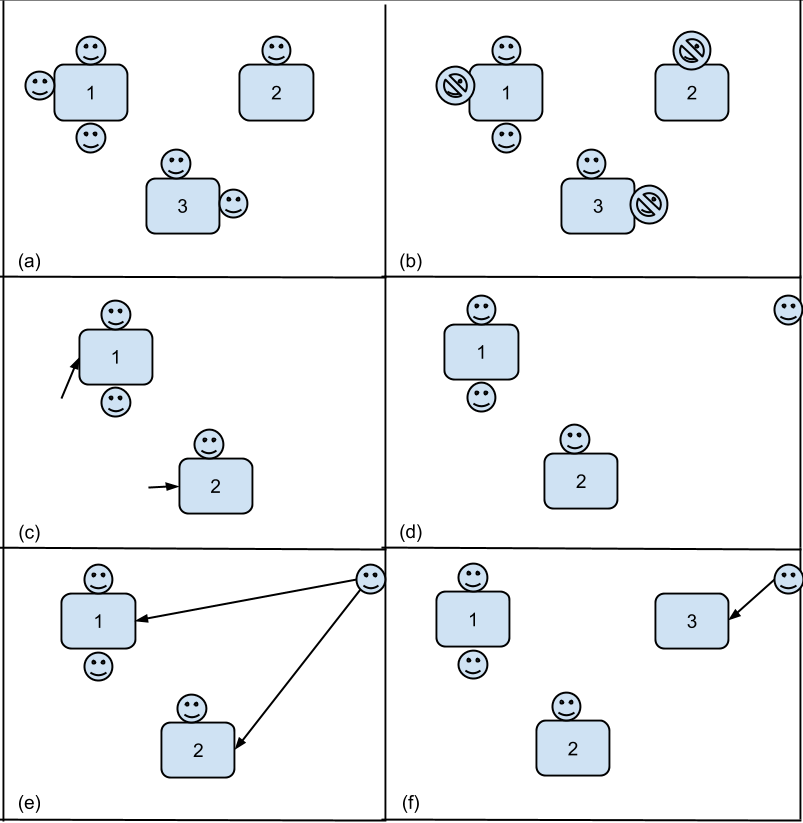
\includegraphics[width=.55\textwidth]{generalPolya}
    \caption{GPU}
    \label{generalPolya}
\end{wrapfigure}

\section{Model definition}
\label{sec:model}

\subsection{General pipeline}

The general flow of operations that shows the communication protocol between the pipeline and the EKF module is presented in Fig.~\ref{pipeline}(a). During step 1, the EKF-SLAM module requests new observation readings given the cloud currently read by the sensors and the position of the robot. The pipeline takes that cloud, extracts clusters and returns the landmarks currently being observed while taking into account landmarks that where observed in the past. Landmarks and clusters are identical concepts representing a different layer in the pipeline. More specifically, clusters are output from the sampler from the sampler and are given as an input of landmarks to the EKF module. Fig.~\ref{pipeline}(b) shows a more detailed view of the computations of the pipeline. The procedure that is shown in Algorithm~\ref{euclid} is described analytical in as follows:




\begin{wrapfigure}{l}{0.7\textwidth}
\begin{tabular}{cc}
  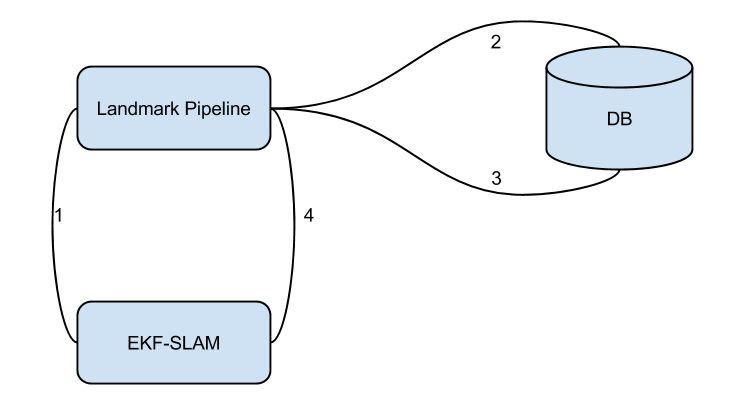
\includegraphics[width=.3\textwidth]{workflowGen} &    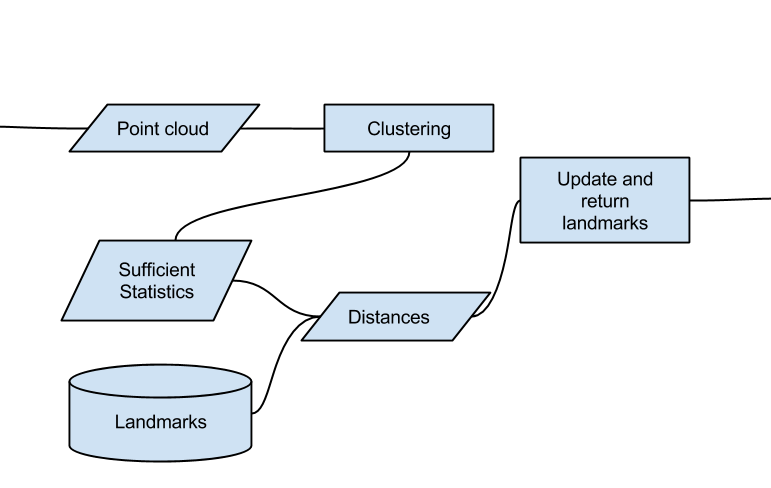
\includegraphics[width=.3\textwidth]{workflowSpec} \\
(a) General pipeline & (b) Landmark pipeline \\[6pt]
\end{tabular}
\caption{General landmark update pipeline}
\label{pipeline}
\   \end{wrapfigure}


\begin{algorithm}
  \caption{Landmark Layer}\label{euclid}
  \begin{algorithmic}[1]
    \Procedure{getLandmarkIds}{$pointCloud, timepoint, existingLandmarks$}
      \State $initialize(landMarkIds)$
      \State $pointCloudReduced \gets extractMetaFeatures(pointCloud)$ 
      \State $features \gets extractMetaFeatures(pointCloudReduced)$
      \State $landmarks \gets cluster(features)$  
      \For{\texttt{$landmarks$ as $landmark$}}
	      \State $ (similarity, landId) \gets calcBestSim(landmark, existingLandmarks) $
			\If{$similarity >threshold$}
			   \State $ addLandmarks(landMarkIds, landId)$
			\Else 
			   \State $ newLandID \gets addLandmarkDB(landmarkDB, landmark)$
			   \State $addLandmarks(newLandID)$
			\EndIf
      \EndFor
      \State \textbf{return} $ landMarkIds$\Comment{Return landmarks}
    \EndProcedure
  \end{algorithmic}
\end{algorithm}


\textbf{Method input:} The method takes as input a point cloud as it is currently being read by the kinect sensor.

\textbf{Lines 3-4:} Feature extraction is done through the pcl\cite{pcl} library. A voxel grid is used to reduce the dataset size. A leaf size of approximately 3cm produces a good trade-off between precision and speed. The object representation used approach is similar to\cite{objectpointslam}. Instead of using the CSHOT descriptor, fpfh\cite{fpfh} histogram is used instead. A fast point feature histogram(fpfh) represents an angular signature between a point and its neighbors. After the fpfh estimation a 23 dimensional angular signature of information between a point and its neighbors is acquired. The final metric that is passed at the sampler is the distance between the histograms of a point and its neighbors. The distance metrics used are EMD,Hellinger,and KL divergence. The color signature of the cloud is being encoded with an approach similar to ~\cite{smcddp}. The color spectrum is discretized and what is extracted is the count of different color signatures between a point and its k nearest neighbors. Finally the position of every point is also given as input to the algorithm. The pipeline is presented in figure Fig.~\ref{pcl:mod}. The pipeline outputs a vector of $ \textbf{x} = (x_s, x_c, x_a) $ of size $l \times 33 $ where $s$ represents a 3x1 vector of space information, $c$ a 27x1 vector of colour information and $a$ angular information. It must be noted that pcl offers a multi threading operation on the point feature histogram extraction. This feature is important since it greatly reduces(6-8 times) the speed of an operation applied on every point of the cloud and that makes the histogram extraction significantly faster.

\begin{figure}[ht!]
  \caption{Point cloud modification pipeline.}
  \centering
    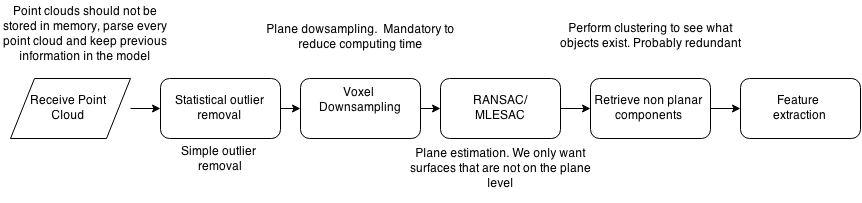
\includegraphics[width=1\textwidth]{Basic}
  \label{pcl:mod}
\end{figure}

\textbf{Lines 5:} The clustering takes place in this line. The input of the method is the feature vector for every data point which is calculated in the previous steps. The clustering is done using the SMC sampler presented in the theory section. 

\textbf{Lines 6-12:} The correspondence of previously seen landmarks to current observations is computed in lines 6-12. Since the landmarks are distributions, statistical distances can be taken to perform the matching. For every observation, its distances with all the stored landmarks are calculated. The calcBestSim function returns the landmark with the highest similarity compared to the one currently being parsed. If the similarity is high enough, correspondence is performed and the landmark is added to the landmark list to be send for update in the EKF, otherwise a new landmark is added and its ID is then added to the list.

\textbf{Lines 15:} The algorithm returns the list of the landmarks the robot encounters in this current timeframe.


Now that the general pipeline is defined, specific parts of the method will be discussed in more detail.

\subsection{The data distribution}
\label{data:dist}

Each point $x$ in the cloud is represented as a tuple $x =(x^s, x^a, x^c ) $ where superscript $s$ represents spatial information, $a$ angle information, and $c$ color information. The method those features are extracted is explained in lines 3 and 4 in the general pipeline. For the purpose of this project each point in the cloud is represented by vector of length 33 with the first three elements representing the space information, elements 4-6 angle information, and the rest color information.

The object model is a mixture of distributions over the data with each object being modeled as D($\theta_t^k$) where $\theta$ represents the parameters of object $k$ at time $t$. More specifically, each set \textbf{x} with $n$ datapoints at time $t$ is distributed as:
$$ x_{t,n} \sim D(\theta_t^k) = Normal(x_{t,n}^s| \mu_t, \Sigma_t) Mult(x_{t,n}^c | \delta_t) Exp(x_{t,n}^a | \lambda_t) $$

Where Normal is a three dimensional Gaussian distribution with mean $\mu$ and covariance $\Sigma$ representing the positional distribution of the data; Mult is a Categorical multinomial distribution with parameter vector $\delta$ representing the weights of the color distribution and Exp is an exponential with shape parameter $\lambda$ representing the angle distribution of the data within the cluster. The exponential distribution was chosen to model angular information after empiric evaluation showed that it would be a good fit for the angle signature distribution of the data. A typical angle signature distribution is shown in.~\ref{pcl:kl}. Since there is a clear exponential trend, the exponential distribution was chosen to model the angle signature of the data.


\begin{wrapfigure}{l}{0.35\textwidth}
    \centering
    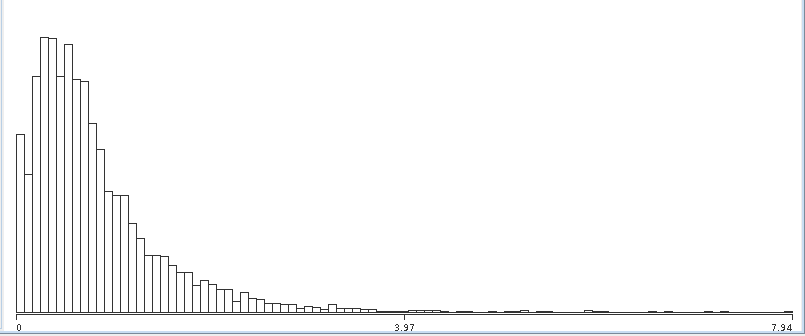
\includegraphics[width=.35\textwidth]{Kullback-Leibler}
    \caption{Exponential trend}
    \label{pcl:kl}
\end{wrapfigure}


Now that the distribution of the objects is defined, the progression of the sufficient statistics at time $t$ given $t-1$ given by:

$\theta_t^k | \theta_{t-1}^k \sim
\begin{cases} T (\theta_{t-1}^k) &\mbox{if } k \leq K_{t-1} \\
G_0 & \mbox{if } k > K_{t-1}. \end{cases}$

Where $T$ represents the transition kernel of the data given the previous state in the model. The case $ k > K_{t-1} $ represents the creation of a new cluster and $G_0$ is the base distribution of the DDP. In our case, the conjugate priors of the distributions of the data were chosen to model the base distribution. Therefore, $G_0$ is defined as:

$$ G_0(\theta_t^k)  = NiW( \mu_t^k, \Sigma_t^k | \kappa_0, \mu_0, \nu_0, \Lambda_0 ) Dir(\delta_t^k | q_0) Gam( \lambda_t^k | \alpha_0, \beta_0) $$

Where NiW is a Normal inverse Wishart distribution, Dir denotes a Dirichlet distribution, and Gam the Gamma distribution. $ \kappa_0, \mu_0, \nu_0, \Lambda_0, q_0,\alpha_0$ and $\beta_0$ are predefined parameters of the model. The generative process for the Dependent Dirichlet mixture model can be written for each timestep $t$ as:

\noindent\makebox[\linewidth]{\rule{\textwidth}{0.4pt}}
\begin{enumerate}
	\item Draw  $c_t$ $\sim$ $GPU(\alpha, \rho) $
	\item $\forall$  k draw: $ \theta_t^k | \theta_{t-1}^k \sim
	\begin{cases} T (\theta_{t-1}^k) &\mbox{if } k \leq K_{t-1} \\
	G_0 & \mbox{if } k > K_{t-1}. \end{cases}$
	\item $\forall$  point $n$ draw $ x_{t,n} \sim F(\theta_t^{c_t,n})$
\end{enumerate}
\noindent\makebox[\linewidth]{\rule{\textwidth}{0.4pt}}
Given the theory in \cite{caron}, the transition Kernel must satistfy:

$$ \int G_0(\theta_k) T(\theta_t^k | \theta_{t-1}^k) d\theta_{t-1}^k =  G_0(\theta_k) $$

The equation means that the invariant distribution must equal its base distribution. A typical way of meeting this restriction and forcing the sampler to converge to the original target density\cite{smc:theory} is to introduce a set of M auxiliary variables \textbf{z} such that:

$$ P(\theta_t^k | \theta_{t-1}^k) =  \int P(\theta_t^k | z_{t}^k)   P(z_t^k| \theta_{t-1}^k) dz_t^k $$

The transition kernel of the model can now be sampled by using the following formula

$\theta_t^k \sim T(\theta_{t-1}^k) = T_2 \circ T_1(\theta_{t-1}^k)$ where:
\begin{equation} \label{eq1}
\begin{split}
z_t^k  & \sim T_1(\theta_{t-1}^k)\\
 & = Normal(\mu_{t-1}, \Sigma_{t-1}) Mult( \delta_{t-1}) Exp( \lambda_{t-1})
\end{split}
\end{equation}

\begin{equation}
\begin{split}
\mu_t, \Sigma_t, \delta_t,  \lambda_t & \sim T_2(z_t^k)\\
 & = NiW( \kappa_0, \mu_0, \nu_0, \Lambda_0 ) Dir(q_0) Gam(\alpha_0, \beta_0) 
\end{split}
\end{equation}

where $\mu_t, \Sigma_t, \delta_t,  \lambda_t$  are posterior parameters given the auxiliary variables $z$.

\subsection{Sequential monte carlo sampler}

Sequential monte carlo samplers for Dirichlet process mixture models where introduced by Doucet et al~\cite{doucet} and serve as fast alternative to MCMC and VI methods of performing posterior inference. SMC samplers have known strengths and weaknesses and are a good fit for the problem at hand, as their main theoretical disadvantage which is the particle degradation is hard to occur at a small time horizon of that the sampler is being used. We can now define the SMC sampler that will be used to perform inference on our model as follows:

\begin{algorithm}[ht!]
  \caption{SMC for DDPM}\label{SMC}
  \begin{algorithmic}[1]
	\State \textbf{Input:} Points \{$x_{1,1:N_t}, ..x_{T,1:N_t}$\}with extracted features
	\State \textbf{Output:} Clusters representing of the data
	\For{$t = 1,...T$} 
			\For{$ l = 1,...L$} 
							\For{$ iter = 1,...S$} 
								\State Sample $(c_t)^{(l)} \sim Q_1$  
								\State Sample $(\theta^k ) \sim Q_2$
						    \EndFor		
		    \EndFor
		    \For{$ k = 1,...K$} 
			   \State Sample $\Delta s_{t-1}^k \sim Binom( (s_{t-1,N_{t-1}}^k)^{(l)}, \rho) $ 
		       \State Set $s_{t,0}^{k} = s_{t-1,N_{t-1}}^{k} -\Delta s_{t-1}^k$
   		       \State Sample $( (z_{t+1}^k)^{(l)} ) \sim T_1((\theta_t^k))^{(l)} $
		    \EndFor
		 	\State compute particle weights $w_t^l$
    \EndFor
    \State Normalize and resample weights
  \end{algorithmic}
\end{algorithm}

\subsubsection{Gibbs updates}
The proposal distribution $Q_1$ is the probability of an assignment $c_{t,n}$ given cluster sizes, parameters and concentration $\alpha$. Formally $Q_1$ can be written as:
\begin{equation} \label{Gibbs}
 Q_1(c_{t,n} | s_{t,n}^k, \theta_t^k, \alpha) \propto Cat( s_{t,n}^1,...s_{t,n}^K, \alpha ) \times
 	\begin{cases} 
 	F(x_{t,n} | \theta_t^{c_t} )  &\mbox{if } k \leq K_{t-1} \\
 	\int P(x_{t,n} | \theta_t )G_0(\theta) d\theta & \mbox{if } k > K_{t-1}. \end{cases}
\end{equation}
Where $c_{t,n}$ represents cluster $c$ of point $n$ at time $t$, $s$ represents cluster sizes. The integral represents the posterior predictive distribution of the cluster times the base distribution with the parameters integrated out. A review of the literature helps understand how the posterior predictive formula is derived. More specifically, the analytic expression of the integral is:


\begin{equation} \label{Q1}
	\begin{split}
		 	\int P(x_{t,n} | \theta_t )G_0(\theta) d\theta =
		 	\int Normal(x_{t,n}^s| \mu_t, \Sigma_t) Mult(x_{t,n}^c | \delta_t) Exp(x_{t,n}^a | \lambda_t) \times  \\ NiW( \mu_t, \Sigma_t | \kappa_0, \mu_0, \nu_0, \Lambda_0 ) Dir(\delta_t | q_0) Gam( \lambda_t | \alpha_0, \beta_0)  d\theta  \\
			= \int Normal(x_{t,n}^s| \mu_t, \Sigma_t) \times NiW( \mu_t, \Sigma_t | \kappa_0, \mu_0, \nu_0, \Lambda_0 )\\
			 Mult(x_{t,n}^c | \delta_t) \times Dir(\delta_t | q_0) \\
			 Exp(x_{t,n}^a | \lambda_t) \times  \times Gam( \lambda_t | \alpha_0, \beta_0)  d\theta  \\
		 	= t_{\nu_0-1}( x_{t,n}^s | \mu_0, \frac{\Lambda_0(\kappa_0+1)}{\kappa_0(\nu_0-1)}) \times \prod_{j=1}^V \frac{\Gamma(x_{t,n}^c)}{\Gamma(q_0)} \times \\ \frac{\Gamma(\sum_{j=1}^V q_0)}{\Gamma(\sum_{j=1}^V x_{t,n}^c)} \times Lomax(\alpha_0 + s_{t,n}^c, \beta_0 \sum_{j=1}^V x_{t,n}^c)
 	\end{split}
\end{equation}

Where $t$ represents student's t-distribution with $\nu$ degrees of freedom, Lomax represents Lomax distribution with shape and scale, $\alpha$ and $\beta$ repsectively and the rest represent a Dirichlet-Multinomial(aka DirMul) distribution. The formulas of the posterior predictive distributions can be found in the literature with \cite{compendium} being a good example. 

The conjugacy of the base and prior distribution allows for an easy sampling formula for proposal distribution $Q_2$ which is of the form: 


\begin{equation} \label{Q_2}
\begin{split}
Q_2(\theta_t^k | \theta_{t-1}^k , x_t^k, z_t^k) \propto F( x_t^k | \theta_k) \times T_2(\theta_t^k | z_t^k) \\
= NiW( \mu_t^k, \Sigma_t^k | \kappa_n, \mu_n, \nu_n, \Lambda_n ) Dir(\delta_t^k | q_n) Gam(\lambda_t^k | \alpha_n, \beta_n)
\end{split}
\end{equation}

With:

\begin{equation} \label{udpates}
\begin{split}
\kappa_n = \kappa_0 + N ,
\nu_n = \nu_0 + N ,
\mu_n = \frac{\kappa_0}{\kappa_0 + N} \mu_0 +  \frac{N}{\kappa_0 + N} \overline{x}^s\\
\Lambda_n = \Lambda_0 + s_{x}^s,
q_N = q_0 +  \sum_n x_i^c,
\alpha_n = \alpha_0 +  N,
\beta_n = \beta_0 +  \sum^n x_i^a
\end{split}
\end{equation}


Where $\overline{x}$ defines the sample mean for the elements assigned at cluster $c$, $s_{x}$ the sample variance and $N$ denotes the number of observations. The formulas for the updates can be found at the literature of cojugate priors like\cite{conjugate}.

\subsubsection{Weight updates}

The only thing left is to define the weight update step. More specifically, on every time step $t$ the weight of particle $l$ is calculated as:

\begin{equation}
w_t^{(l)} = \frac {P(c_t^{(l)} , \theta_t^{(l)}, x_t| 	\theta_{t-1} )}{P(c_t^{(l)} , \theta_t^{(l)}| 	\theta_{t-1} )}
\end{equation}

Using Bayes rule, the numerator can be written as:

\begin{equation}
	P(x_t , | c_t^{(l)} , \theta_t^{(l)} \theta_{t-1} ) \times P(c_t^{(l)} , \theta_t^{(l)}|  \theta_{t-1} )
\end{equation}

Which can be calculated using equations $Q_2$ and $Q_1$ for the first and second part respectively. After the particle weights are normalized particles are drawn with probability proportional to their weights.

\subsection{Decision Layer}

Once the sampler outputs the clusters of the point cloud the output can be passed to the decision layer. The decision layer calculates how similar a cluster is to clusters encountered before, and if the similarity is high enough the clusters are considered to be part of the same landmark. To do that, distance measures must be defined between the stored clusters and the ones that are inferred at the current iteration of the algorithm. Distances between distributions are called divergences and a large amount of literature on divergences exists.

Every cluster consists of a three part distribution as it was defined in section \ref{data:dist}. To define a distance measure between cluster, individual distances between all the distribution parts will be defined. More specifically let $l$ be the distribution of the cluster and $o$ the distribution of a currently observed cluster. $l$ and $o$ can be decomposed into 3 parts: $l_G$,$l_C$,$l_E$ where G,C and E stand for Gaussian, Categorical and Exponential respectively. With that notation the distances between those distributions can be defined. For each individual landmark distribution $l$ and observation distribution $o$ the distances computed where the following:

\begin{itemize}
	\item Wesserstein($l_G,o_G$);			
	\item Kullback-Leibler($l_G,o_G$);
	\item SquaredHellinger($l_E,o_E$);
	\item Kullback-Leibler($l_E,o_E$);
	\item Kullback-Leibler($l_C,o_C$);
\end{itemize}

With that in mind the distance between every distribution can be transposed of a vector of length 5. That way, deciding if a cluster is part of a landmark that has been encountered before is now a problem of finding the optimal decision boundary given the distances at hand. For the purposes of this thesis, the decision boundary of an observation being a landmark or not was chosen by empiric evaluation of the landmarks. It is of course possible to learn the optimal decision boundary but due to time restrictions a simpler decision making approach was chosen instead.

\subsection{Complexity}

The complexity can be decomposed into three parts. The cloud downsampling, the clustering and the decision making process.
$$
O(total) = O(filter) + O(cluster) + O(decision)
$$
\textbf{Downsampling}: The complexity of the cloud downsampling pipeline can be decomposed to the one of its components. This means that the decomposed complexity is defined as follows:
$$O(filter) = O(Downsampling + Stat\ Removal + RANSAC+ FPFH + Color\ est) $$

Voxel downsampling searches for neighbors within a distance defined by the user and keeps an average value that equally represents the cloud. Since the operation involves searching for neighbors of a point, and since search operations take $O(log\ n)$ time where N is the number of points within the cloud, the complexity of voxelGrid downsampling is $O(k log n)$ where $k$ is the number of neighbors and $n$ the number of points in the cloud. It is reasonable to assume that the averaging operations take $O(1)$ time since they can be done while searching.
Statistial outlier removal searches for k nearest neigbhors and removes those whose deviation is passed a certain threshold. Given that search operations take $O(log\ n)$, for k neighbors, the complexity is $O(k\ log\ n)$. The same assumption regarding the averaging computations is done here.
A high amount of research has been done regarding the optimal complexity of RANSAC~\cite{RANSAC}. RANSAC has a complexity of $ O(k+ m_s*N)$ where k is the maximum amount of iterations defined by the user, $m_s$ the average number of models per sample $N$ the number of data points.
FPFH operations have a complexity of $O(nk)$ as given in~\cite{fpfh}.
Finally, for the operation of color estimation, the k nearest neighbors are chosen and some constant operation is performed on them. The complexity here is similar to Statistical outlier removal since operations after the search are assumed to take take $O(1)$ time. The complexity for color estimation then becomes $O(k\ log\ n)$ where $k$ is the number of neighbors, $n$ the number of points. 

The downsampling pipeline has a total complexity of:
\begin{equation} \label{Q_filt}
O(filter) = O(k_{0}\ log\ n_{init} + k_{1}\ log\ n_{1} + k_{2}+ m_s*n_{2} + n_{3}k_{3} + k_{4}\ log\ n_{3} )
\end{equation}

Different $k$ indexes represent the number of neighbors defined for every operation. The $n$ represents the number of points used as input. Using the notation  of equation \ref{Q_filt}, $n_{init}$ defines the whole cloud, $n_1$ the cloud after operation 1, $n_2$ the cloud after operations 2 etc.

\textbf{Clustering}: The complexity of the SMC sampler is defined in \cite{smcddp} as $O(TLKSN)$ where $T$ defines the time frames, $L$ the number of particles, $K$ the number of clusters, $S$ the number of samples, and $N$ the size of the dataset. Given that the sampler is only used in single timesteps, the computational complexity is reduced to $ O(LKSN) $. This is a low complexity and directly affects the performance since the sampler averages 10msec of excecution time.

$$
O(cluster) = O(LKSN)
$$

\textbf{Decision making}: The decision making takes $ O(\kappa * l^2) $ computational time where $\kappa$ defines the number of clusters output by the sampler and $l$ the number of landmarks currently stored in the database. This number can be further reduced by taking for example only landmarks that are nearby the cluster, but optimizing the decision making performance is outside the scope of this project.


Finally, with some notation abuse, the final complexity of the method can then be defined as:

\begin{equation} \label{complexity}
\begin{split}
O(filter) + O(cluster) + O(decision) = \\
O(k_{0}logn_{0} + k_{1}logn_{1} + O(k_{2}(t_M)+ m_s*n_{2}) + n_{3}k_{3} + k_{4}logn_{3} ) + O(LKSn_3) + O(\kappa * l^2)=\\
O(k_{0}logn_{0} + k_{1}logn_{1} + k_{2}(t_M)+ m_s*n_{2} + n_{3}k_{3} + k_{4}logn_{3} + LKSn_3 + \kappa * l^2)
\end{split}
\end{equation}

The complexity as defined in equation~\ref{complexity} depends greatly on the initial reduction of the voxel downsampling. As the voxel leaf size parameter decreases and the downsampling outputs a larger cloud, the precision as well as the computing time of the method increases. Since in this thesis the research was directed towards online SLAM methods, the leaf size was modified so that the cloud the time requirements for online landmark tracking were met.

\subsection{Landmark size}

The basic block of this algorithm is a cluster containing an environment signature. In order to be able to compute how scalable the method is, the size of a single landmark will be computed. Each landmark is represented by a single row in an SQLite database. To calculate how much space a landmark occupies, we will first calculate how space each of the columns has. Each row consists of 32 real numbers and 1 auto increment integer. Given that SQLite databases assign the memory dynamically, the worst case scenarios will be taken into account so that every other case is also included. According to the SQLite manual of datatypes~\cite{sqlite} a real value takes up to 8 bytes of memory. An auto increment integer takes up to 4 bytes of information, so the total number  of memory for a worst case scenario landmark is 260 bytes. This number can vary greatly over different environments and is a safe assumption to calculate the memory this method occupies.

\section{Results}
\label{sec:results}

\subsection{Simple datasets}

In this section the algorithm will be tested against a simple dataset. That will make easier the conceptual extension to more complex clouds that will be used when mapping the environment. In order to test the sampling as well as the decision layer of the algorithm, a simple dataset provided by the pcl\cite{pcl} library was used. More specifically, a cloud consisting of two milk cartridges with different colors and poses where used. The initial cloud is shown in Fig.\ref{pcl:clust}(a). The cloud was given as input to the downsampling pipeline. The reduced cloud was then passed as input to the sampler and the clustering results are shown in Fig.\ref{pcl:clust}(b).

\begin{figure}
\begin{tabular}{c}
  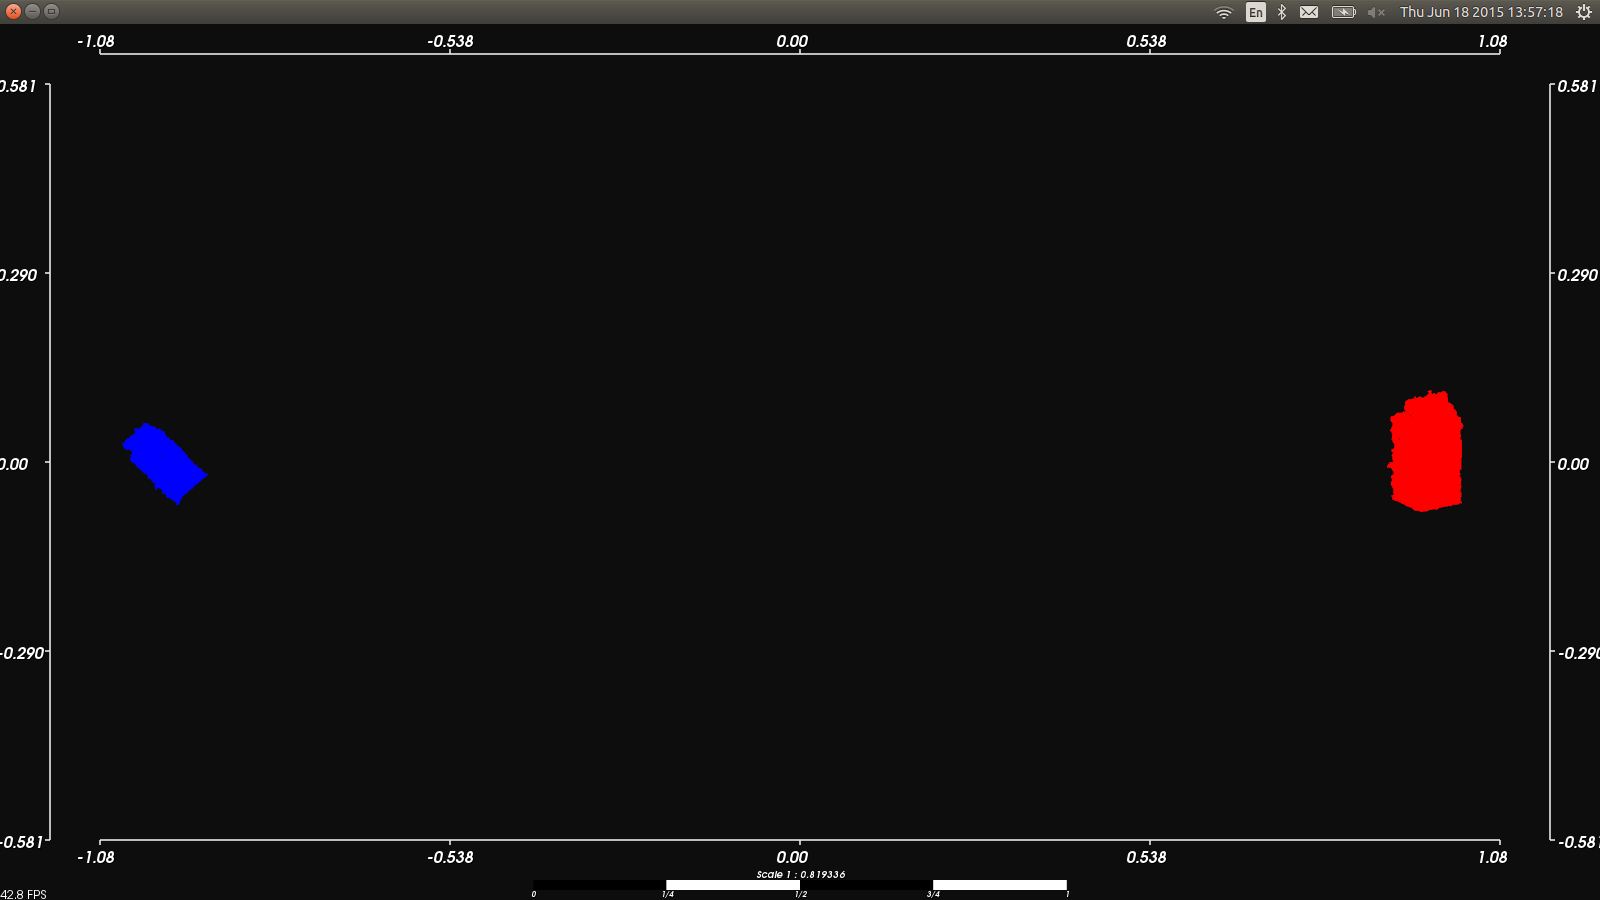
\includegraphics[width=1\textwidth]{clusterings/initialData} \\
  (a) Raw cloud  \\
   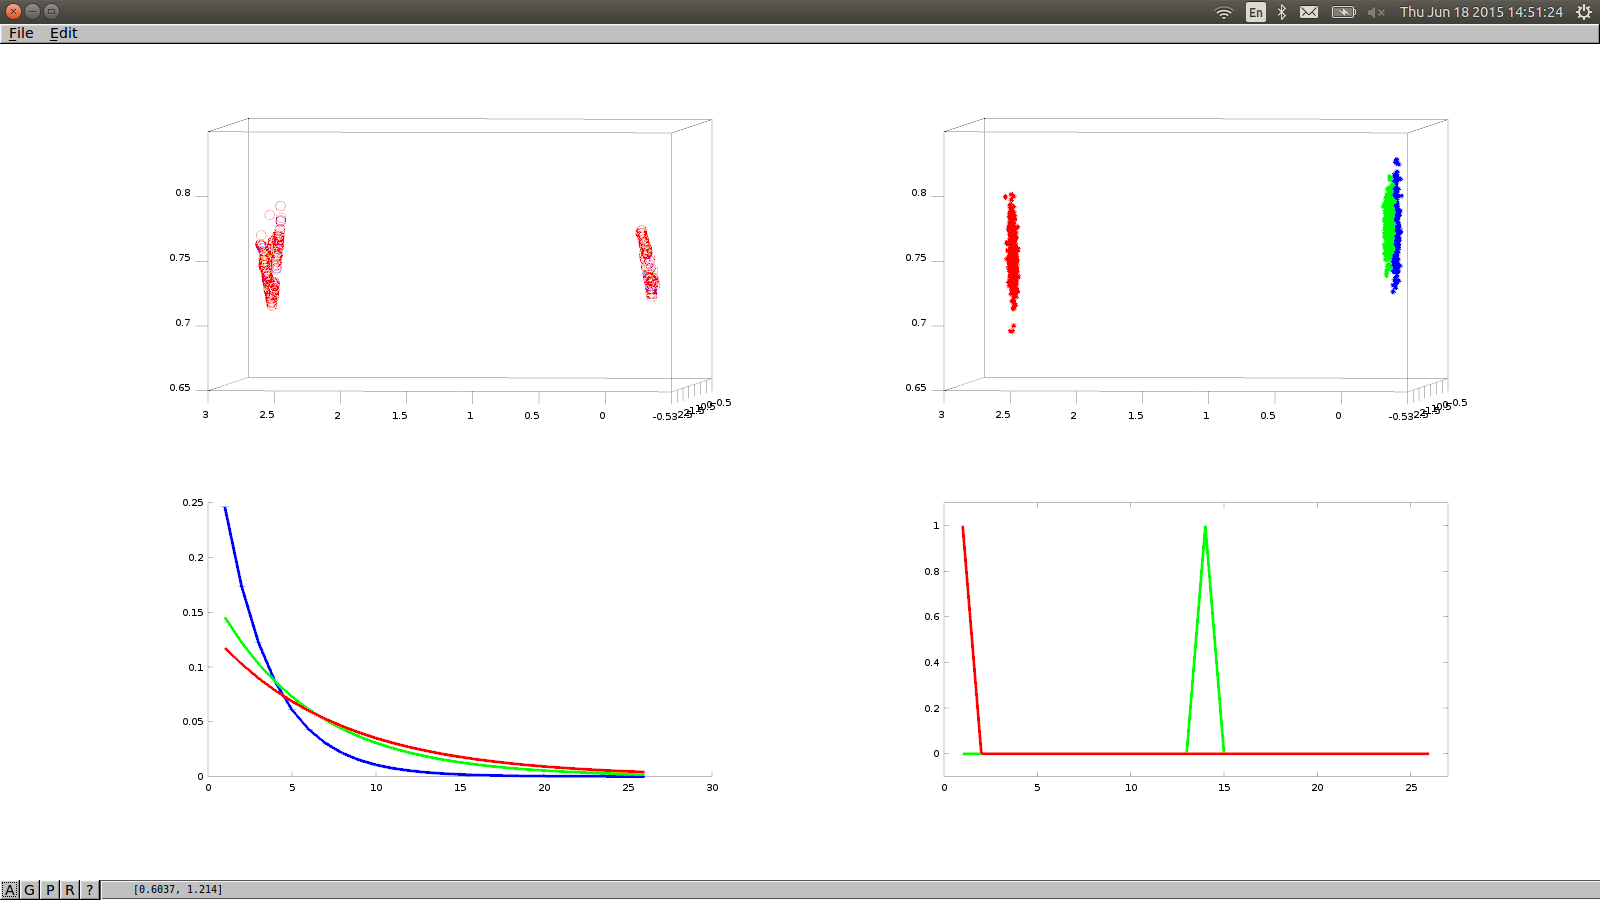
\includegraphics[width=1\textwidth]{clusterings/colorcodedDistributions} \\
 (b) Post clustering \\[6pt]
\end{tabular}
\caption{Initial data along with the distributions infered}
  \label{pcl:clust}
\end{figure}

More specifically, the reduced point cloud is shown in the top left part. It is significantly smaller in size and this cloud along with all the meta-information needed to perform the clustering are given as input to the sampler. The sampler outputs a mixture of distributions that best fits the input data. The clustering output is shown in Fig.\ref{pcl:clust}(b) with the top right being the Gaussian distributions inferred, bottom left the exponential and bottom right the categorical representing the color information of the cloud. The height of the objects leads to distribution with high variance in the z axis. The sampler outputs 3 clusters for the data and it can be seen that the change in angular information of the box leads the sampler to assign two distributions in the left milk box cloud. The color information is captured correctly in the structures and that was expected since the data had distinct colour signatures.

\begin{center}

    \begin{tabular}{|C|C|C|C|C|C|}
    \hline
    \multicolumn{6}{|l|}{\centerline{UUID 1}} \\
    \hline
     LandUUID & GausKL & GausWes & ExpHel & ExpHel & CatKL \\
     \hline
	 1&0&1.18111e-07&0&0.164045&0 \\
	 \hline
 	 2&0.0115821&53.5171&1.20726&0.319589&0 \\
 	 \hline
	 3&13.5579&22449.9&1.56956&0.376699&13.8155 \\
	 \hline
    \multicolumn{6}{|l|}{\centerline{UUID 2}} \\
    \hline
	 1&0.0115821&20.1454&1.7215&0.319589&0 \\
	 \hline
	2&5.42101e-20&4.88951e-08&0&0.411668&0 \\
	\hline
	3&12.8379&21458.6&0.474719&0.449769&13.8155 \\
	 \hline
    \multicolumn{6}{|l|}{\centerline{UUID 3}} \\
    \hline
	 1&13.5579&31191.5&2.55205&0.376699&13.8155\\
	 \hline
     2&12.8379&65013.8&0.53855&0.449769&13.8155\\
     \hline
	3&0&2.43346e-07&0&0.481313&0\\
	 \hline
	 \end{tabular}    
\end{center}

Now that the structured is inferred, the distances between the clusters can be calculated. The table shows the distances between every cluster. It can be seen that the first two landmarks have small distances in their Gaussian counterparts since they represent nearby areas and objects in the cloud that are very far apart. The angular distances between them are also not very large. The distinct colors of the milk boxes make the color signatures of the clusters distinct. An example with more complex color signatures is shown in Fig.[\ref{pcl:clust2}]. The clouds are now given a mixture of colors and this is passed to the color signature inferred on every cluster in Fig.[\ref{pcl:clust2}](b)

\begin{figure}
\begin{tabular}{c}
  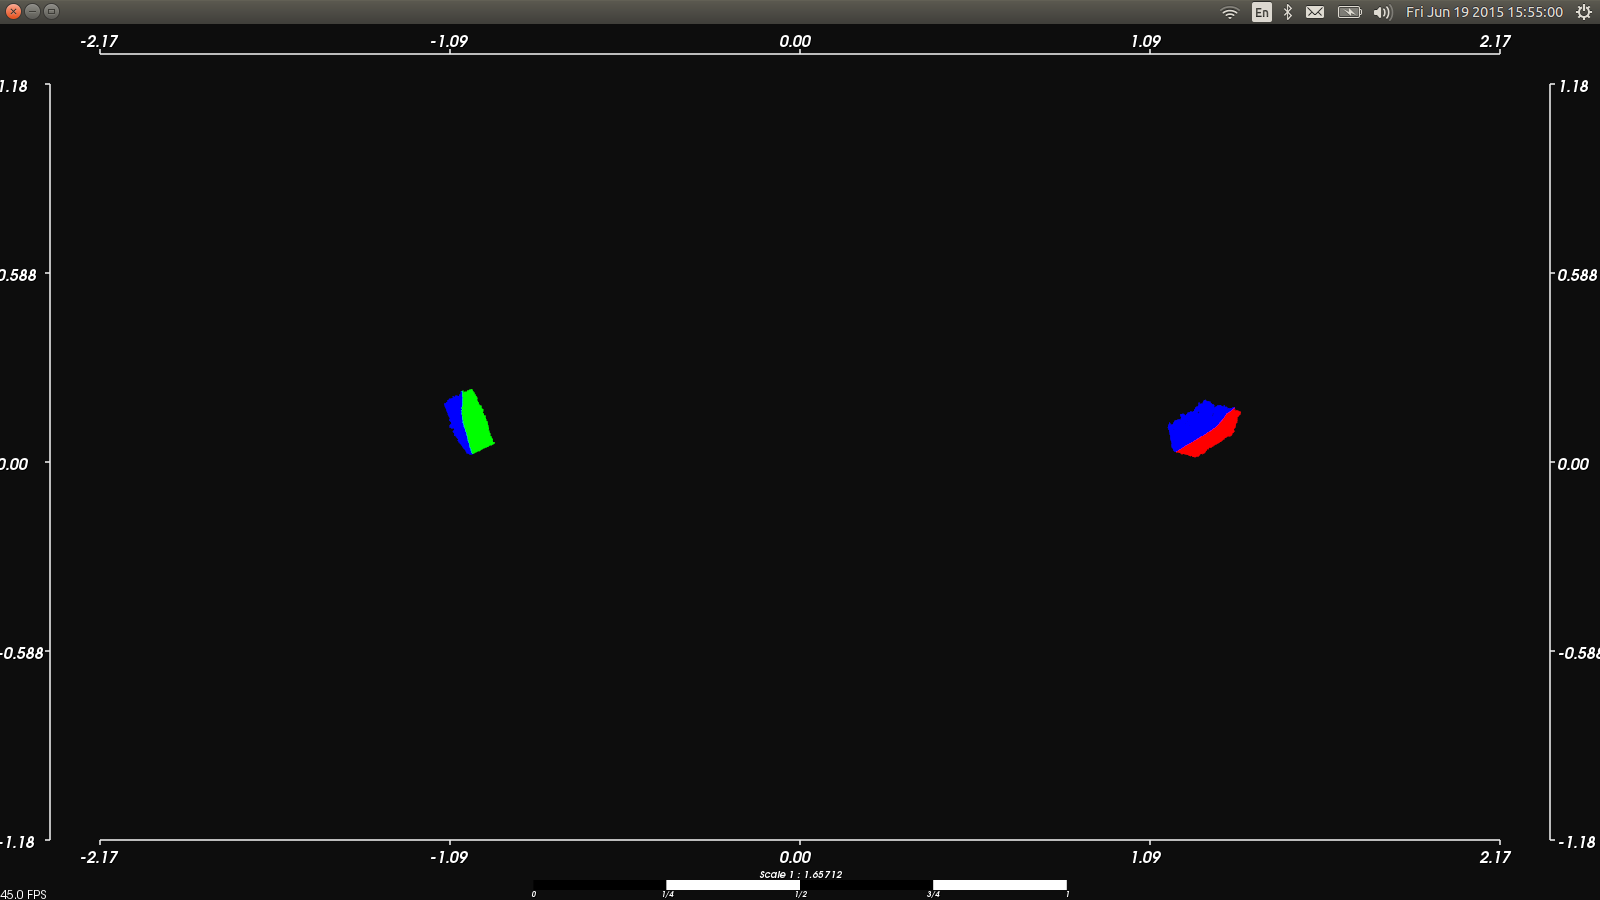
\includegraphics[width=1\textwidth]{clusterings/coloursSource} \\
  (a) Raw cloud  \\
   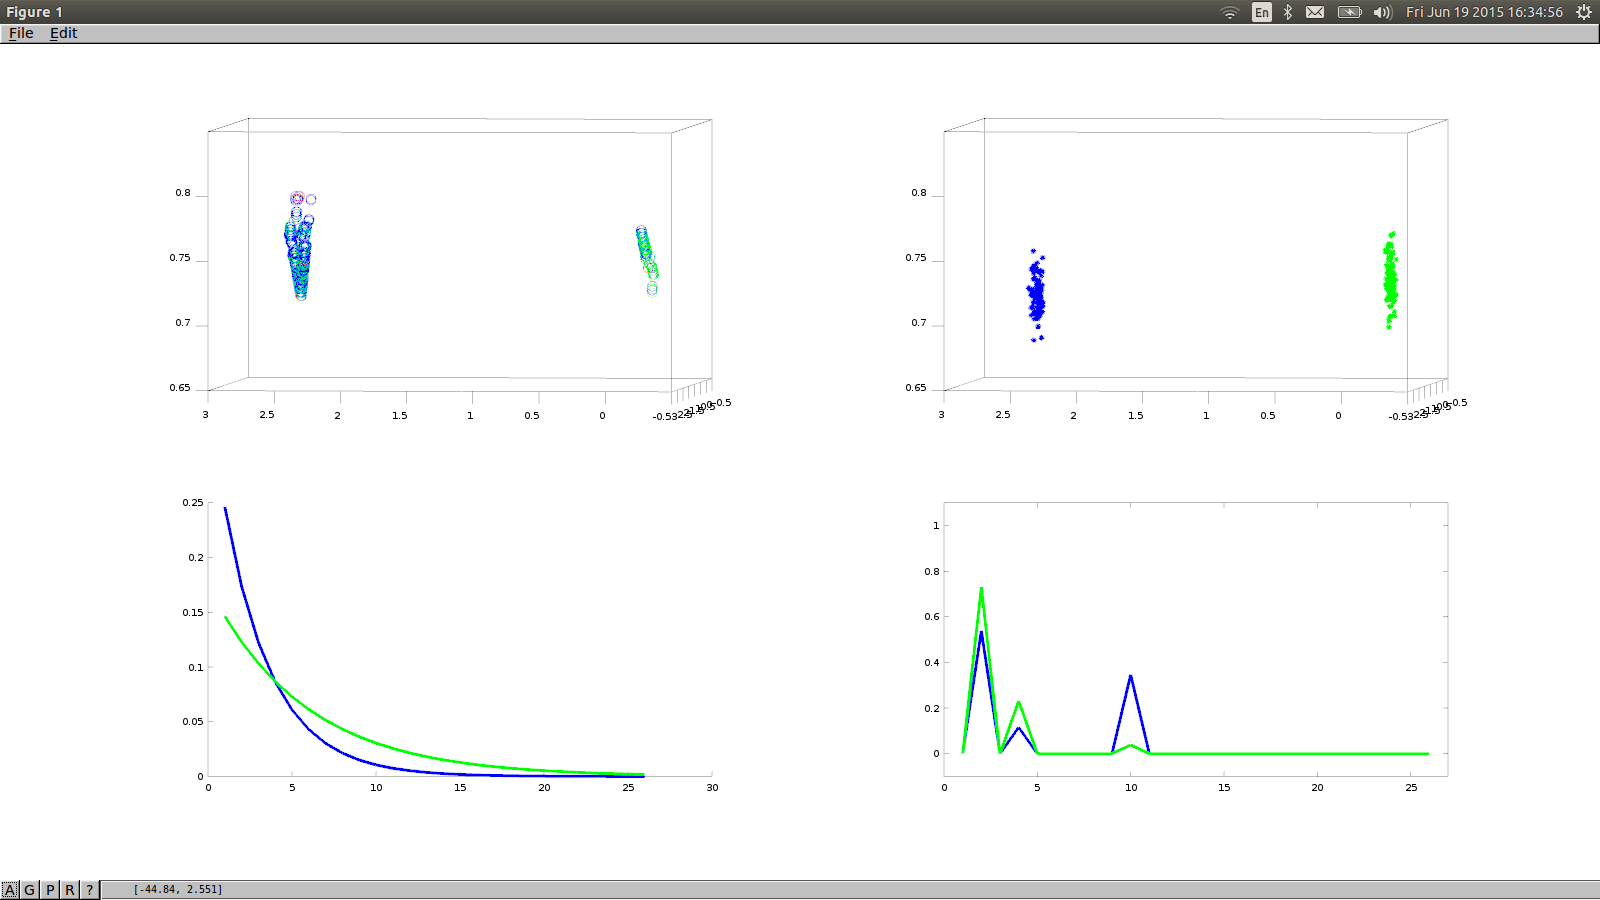
\includegraphics[width=1\textwidth]{clusterings/coloursCorrect} \\
 (b) Post clustering \\[6pt]
\end{tabular}
\caption{More complicated color distributions}
  \label{pcl:clust2}
\end{figure}

\subsection{The decision layer}

The decision boundary of the pipeline can be decomposed into three basic parts; a positional, a color and an angular boundary. Figure[\ref{pip:bounds}] shows the behavior of the decision layer with respect to the Gaussian(positional) and Categorical(color) parts. 

\begin{figure}[ht!]

\begin{tabular}{cc}
  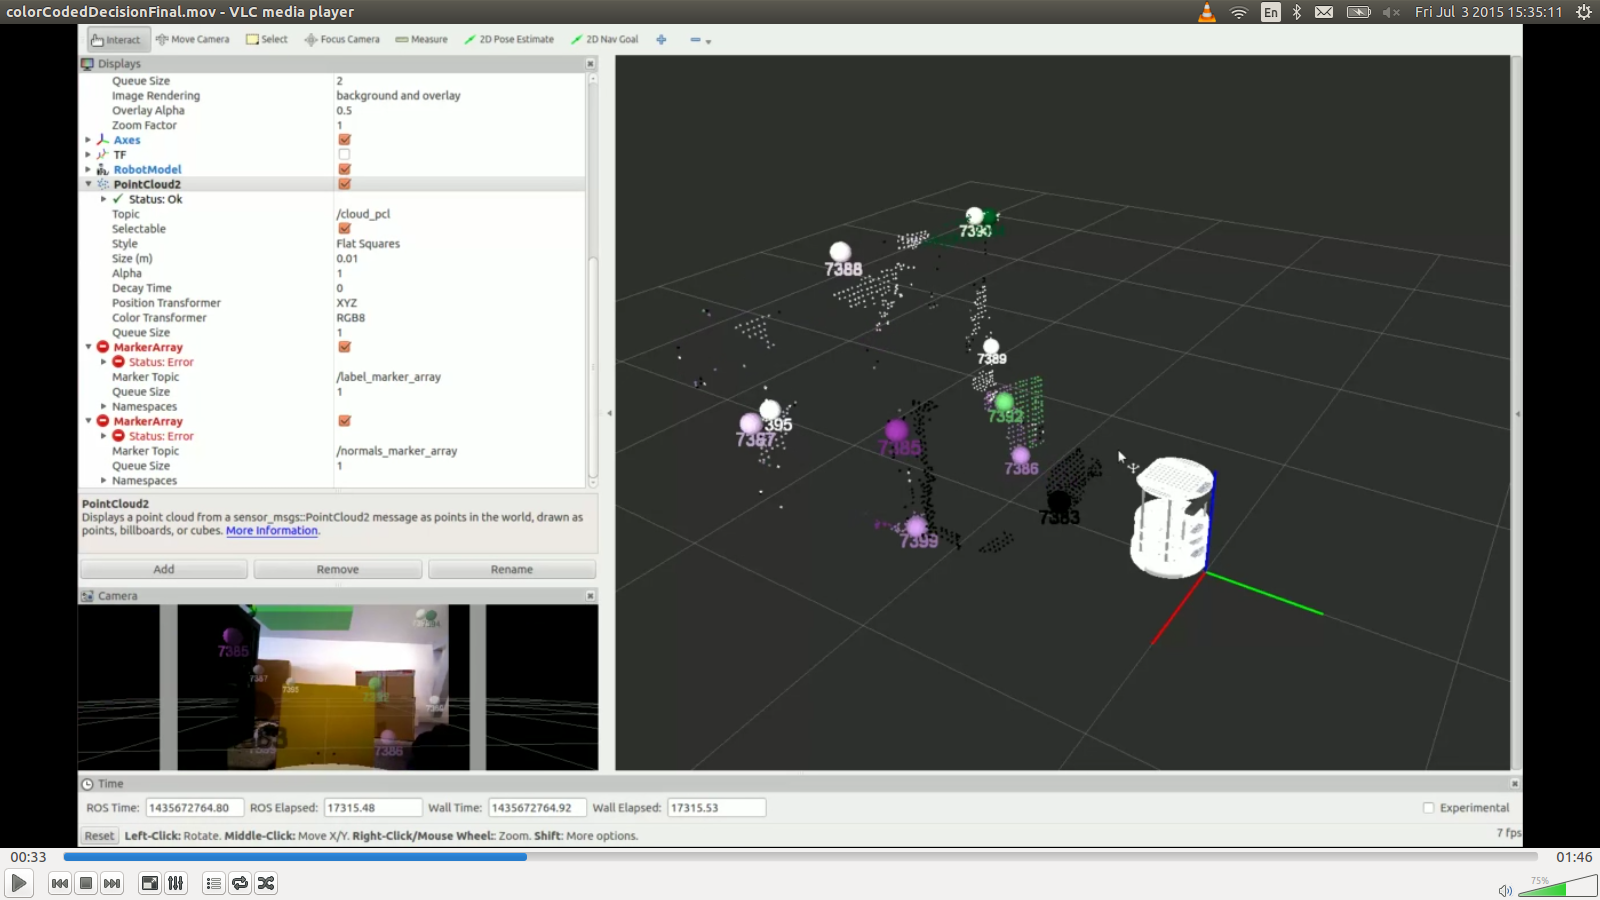
\includegraphics[width=.5\textwidth]{colorBound} &   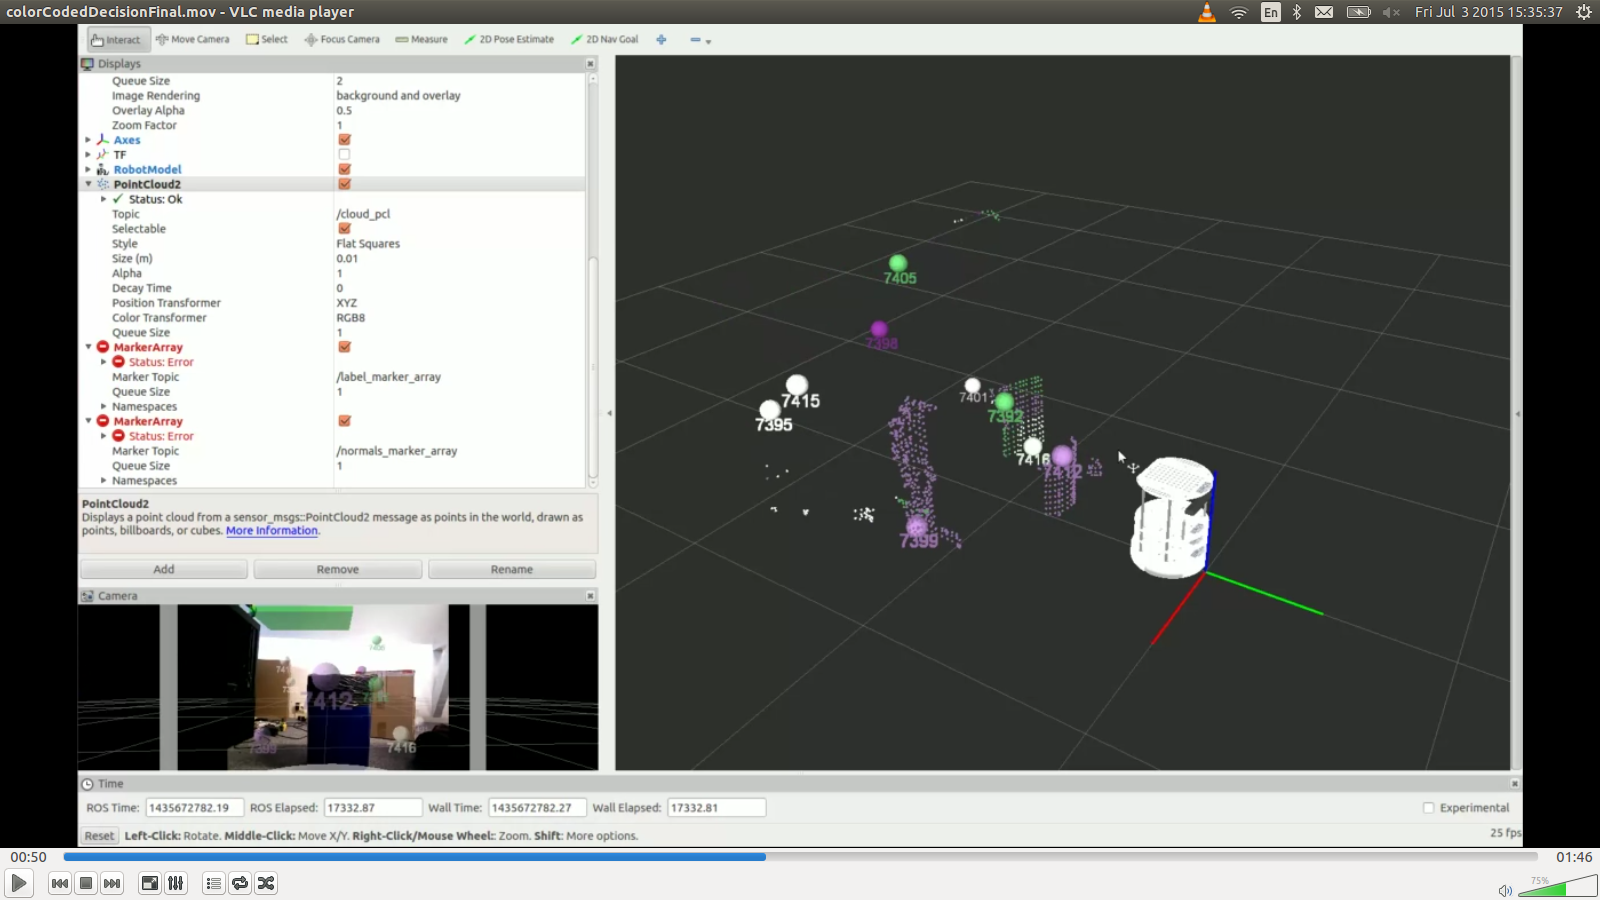
\includegraphics[width=.5\textwidth]{colorBound2} \\
(a) Yellow Folder assignment  & (b) Blue trashcan assignment \\[6pt]
	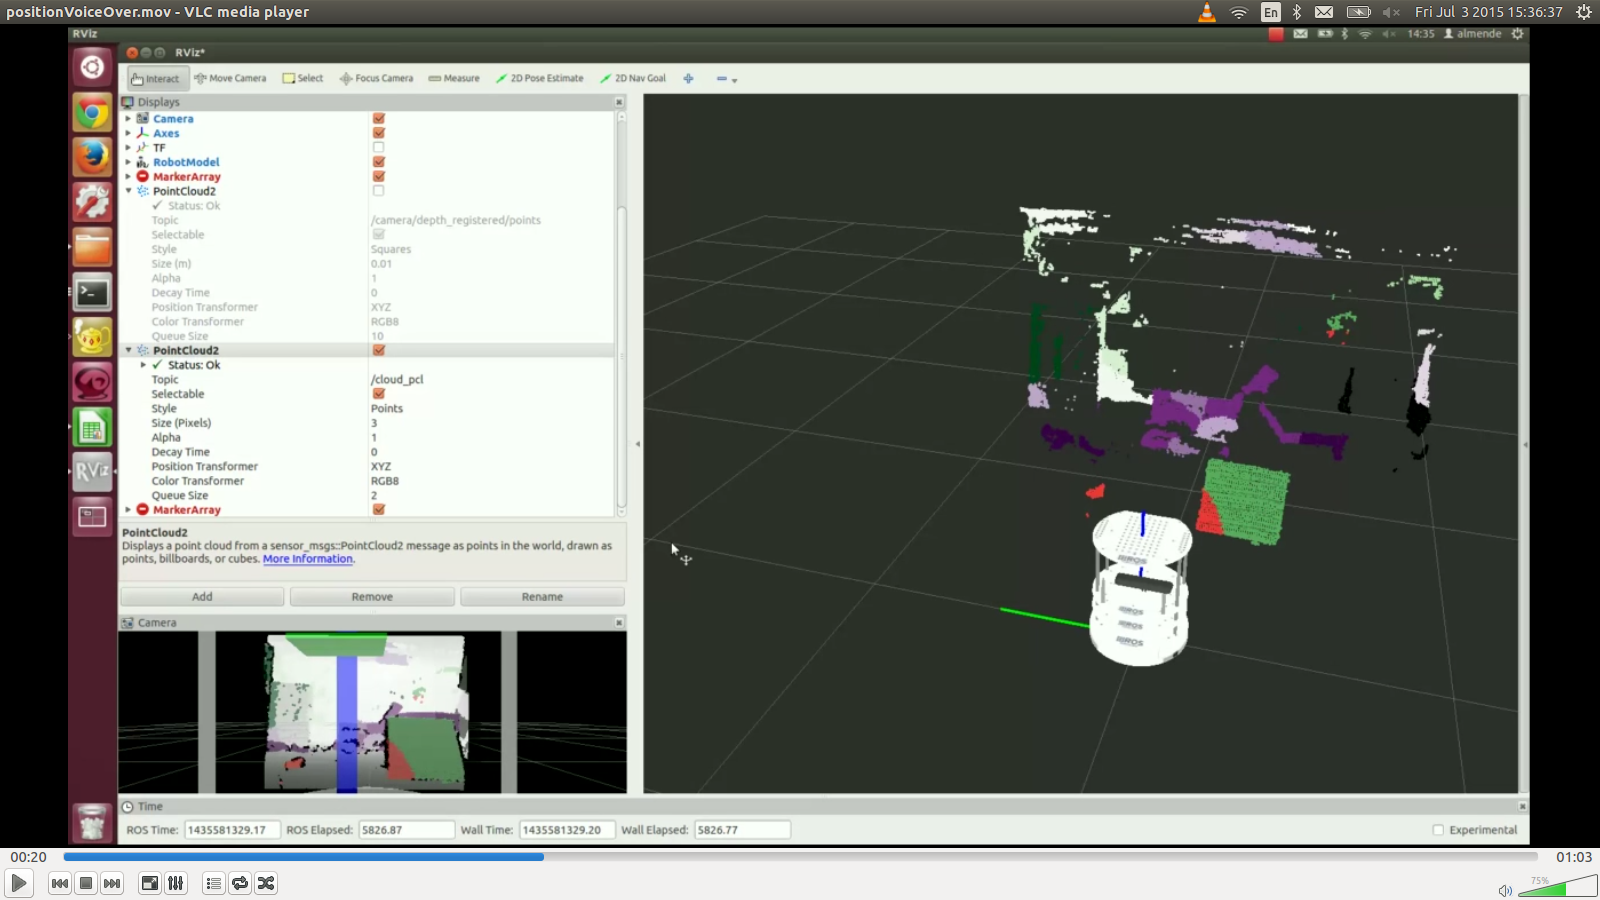
\includegraphics[width=.5\textwidth]{posBound} &   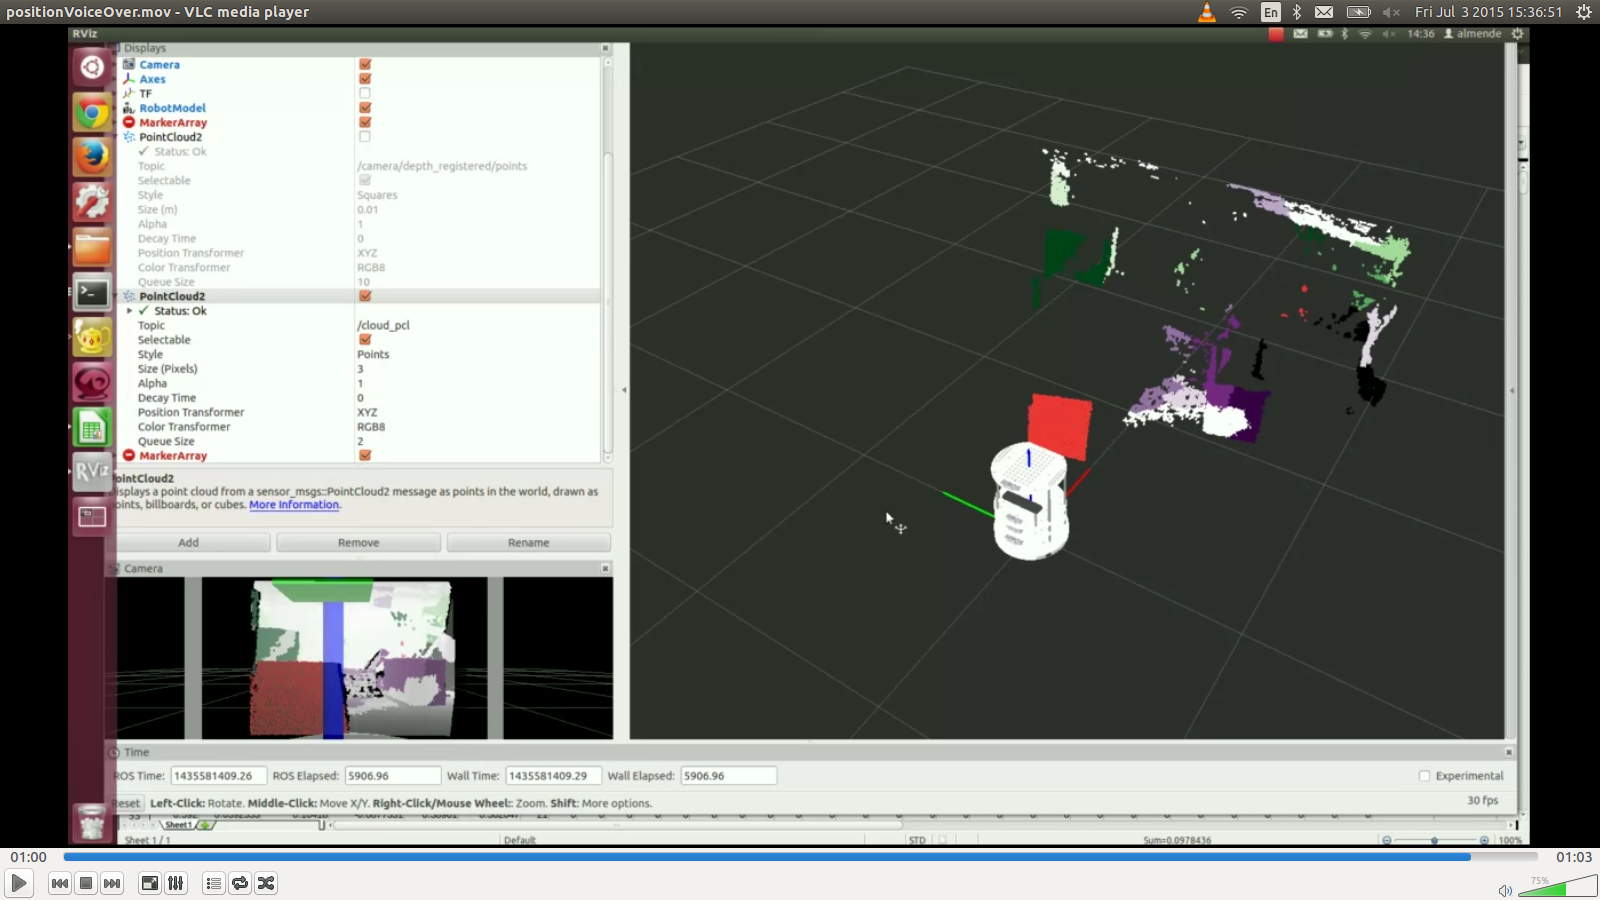
\includegraphics[width=.5\textwidth]{posBound2} \\
(c) Folder initial  & (d) Folder moved \\[6pt]
\end{tabular}
\caption{The colour and position boudnary is displayed in these pictures}
  \label{pip:bounds}
\end{figure}

In Fig.\ref{pip:bounds}(a) the yellow folder allong with some of its environment to the left are being assigned to landmark with id 7386. The folder is then removed and a blue trashcan is put in its place. The folder and the trashcan are similar in size and due to that their Gaussian counterparts will not have large distances. Their main difference lies in the color signature they carry. Since the distance in their color is substantial, a new landmark with id 7412 is created to capture the change in the signature of the environment at that place of the map. The different landmark assigned to the cluster can be seen in Fig.\ref{pip:bounds}(b). In Fig.\ref{pip:bounds}(c) and(d) the positional decision boundary is displayed. In the initial position as shown in Fig.\ref{pip:bounds}(c) the yellow folder is assigned to the green landmark of the cloud. As the object is moved a different position in the cloud, it is being assigned to a different cluster. The reason the cluster is assigned to multiple landmarks is due to the fact that the folder is decomposed to several clusters and each one of them is being assigned to a different part of the cloud with respect to their position. This can be seen in Fig.\ref{pip:bounds}(c) where the bottom left of the folder is being assigned to the red cluster. Parameter tweaking is possible but the purpose of a general pipeline is to use as little parameter tweaking as possible so that the method is general and can easily be applied to a different scenarios.

The exponential part of the distribution is responsible for the angle signature elements within a cluster have. Practically, having a large amount of different angle distributions in a single cluster leads to objects that have texture and their surface is not smooth. Having a very strict limit in the angle distribution can lead to very small clusters and subsequently to a high amount of landmarks within the data. Using the data from the kinect camera, angle distributions are highly prone to high amounts of noise that is found in parts of the cloud that are near the end of Kinect sensor's range. Practical evaluation has shown that using an angle limit that is close to the average distance between angle signatures produces stable results and reasonably sized landmarks in the cloud.


\subsection{Limits of the method}

	Restrictions imposed by the method can be categorized to two major classes. Restrictions to the clustering layer and restrictions to the decision layer of the sampler.


\subsubsection{Clustering layer}


An important limit of the pipeline exists with respect to the Dirichlet hyper-parameter $\alpha$. During the clustering, choosing a correct value for the hyper-parameter $\alpha$ is very important in order to have optimal results. Having sampler run with a very low $\alpha$ can lead to the whole cloud being assigned a single cluster. Having every point in the cloud being part of the same cluster leads to a a significant amount of information loss as no environment specific information are incorporated to the cloud. Fig.[\ref{pip:limits}](a) shows the behaviour of the sampler for $\alpha$ values lower than 1. On the other hand, having a very large $\alpha$ can lead to a very large amount of clusters being output by the sampler every time. That in combination with the stricter decision layer can lead to a non-converging pipeline since every time a new landmark that does not fit the landmark database is output. This leads to many small clusters that contain a small number of points each. Furthermore, having a high value in the hyperparameter leads to a slower sampling procedure since the complexity of the sampler is $O(TKLSN)$ where $K$ is the number of clusters. Fig.[\ref{pcl:kl}](b) displays the behavior of the sampler for very large values $\alpha$.


\begin{figure}
\begin{tabular}{cc}
    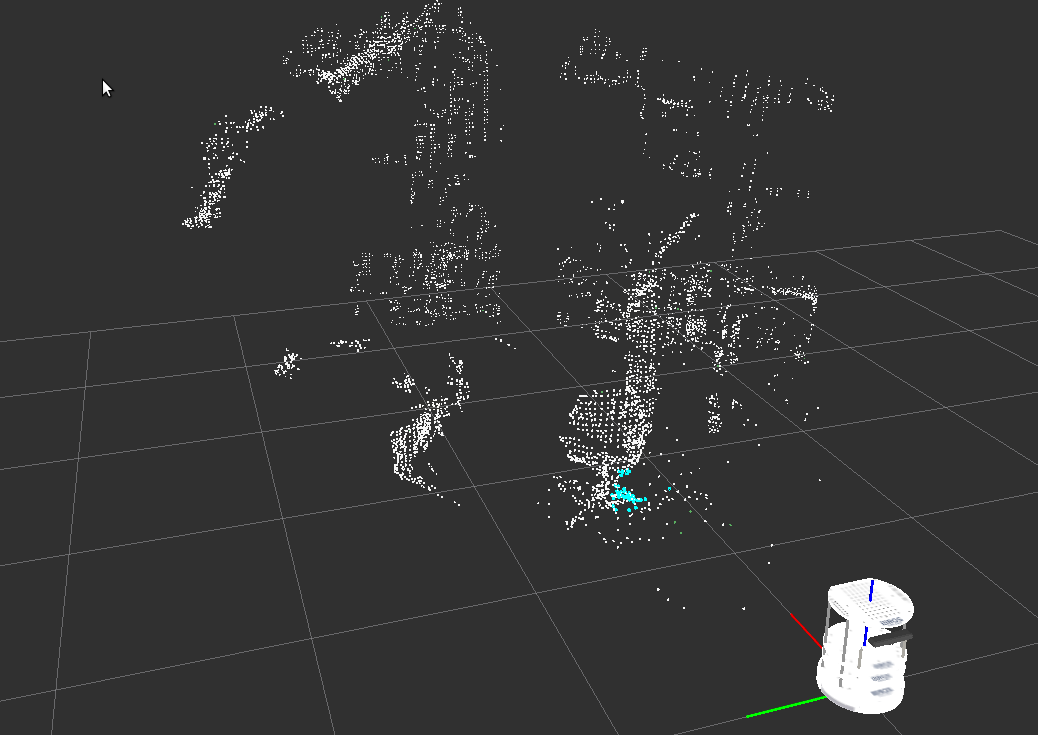
\includegraphics[width=.5\textwidth]{singlecluster} &  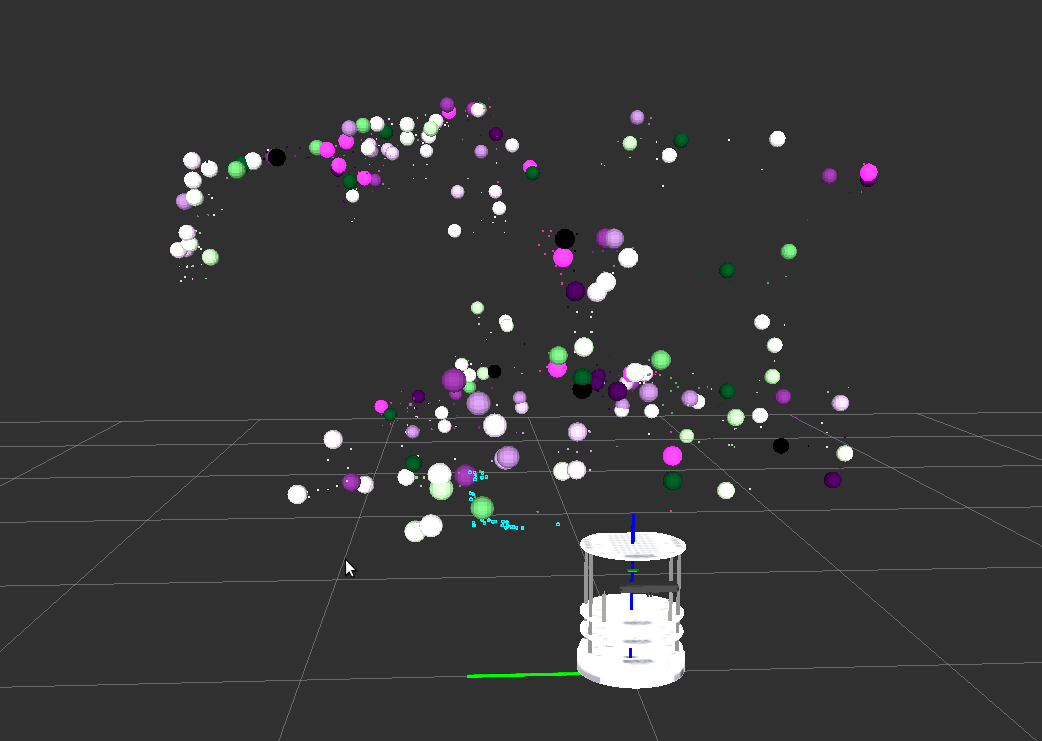
\includegraphics[width=.5\textwidth]{onlyclusters2} \\
  (a) Low $\alpha$ translates to a single cluster  & (b) High $\alpha$ translates to a non converging cloud \\[6pt]
\end{tabular}
\caption{Fail use cases.}
  \label{pip:limits}
\end{figure}

\subsubsection{Decision layer}

The restrictions introduced by the decision layer are relatively simple due to its constant nature. Taking very small distances in the distance threshold operation can lead to pipeline that continuously adds new landmarks to the database. An example is shown in Fig.~\ref{pip:expo} where limiting the landmark matching operation to very small exponential distances, leads to a cloud where objects are decomposed to a lot entitites. It must be noted that the object decomposition is even more intense when camera movement is involved due to the different angles. Furthermore, since the number of landmarks is also a function of noise, areas of the cloud that are near the maximum range of the sensor can lead to different landmarks added frequently. These issues can be tackled by having a less strict limit in the operation that defines what is considered a landmark the sampler has encountered before or not.

    \begin{figure}
        \centering
	    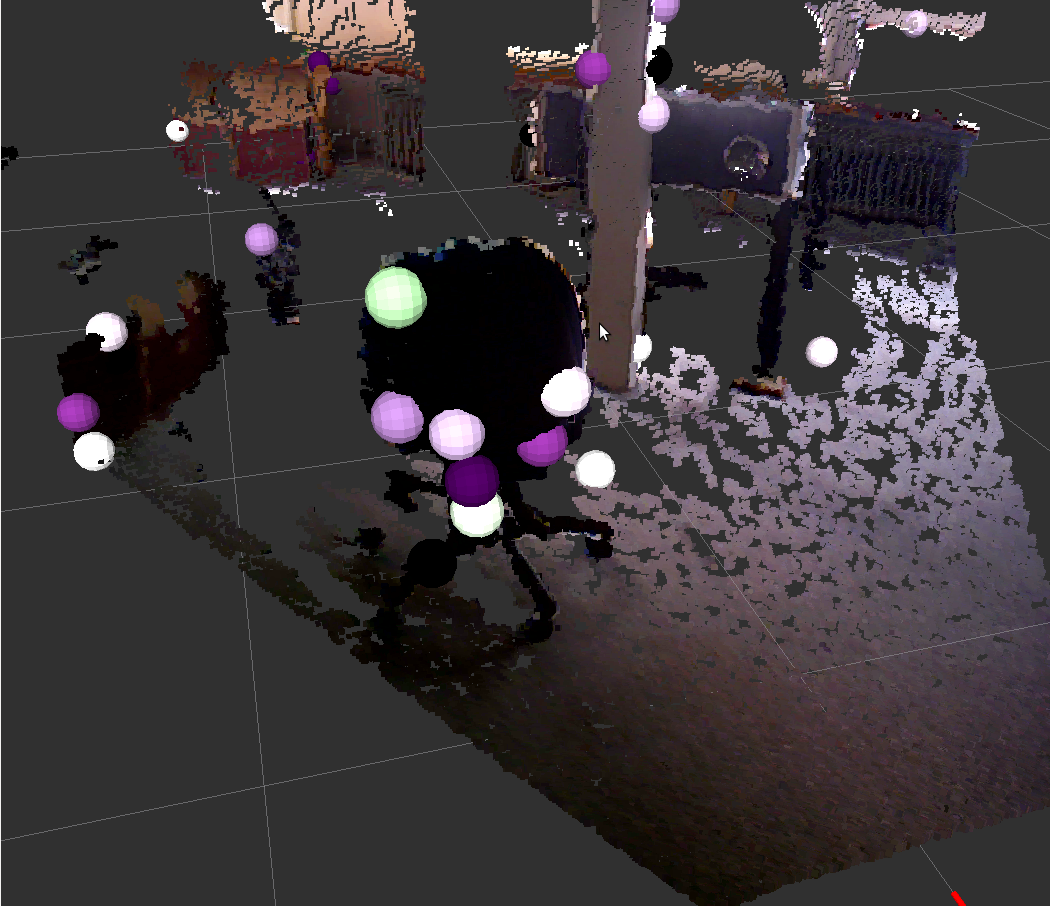
\includegraphics[width=.5\textwidth]{monsterchair} \\
	  (a) Very strict decision limits lead to multiple \\
	   entities on single objects \\[6pt]
	  \label{pip:expo}
    \end{figure}


\subsection{EKF-SLAM experiments}

Finally, the pipeline was used in real life scenarios as a sensor model in a Landmark based EKF SLAM algorithm and was tested in its speed and memory requirements. As it was shown when calculating the complexity of the method, speed is dependent to the downsampling process. If the downsampling threshold operations are strict and the cloud is being stripped of many of its points, accuracy will decline and speed will increase. As shown in the landmark size section, the unit cost of a Landmark has an upper limit. Therefore, the memory requirements of the method are directly depending on how many landmarks the algorithm allows. A strict landmark matching decision layer that requires a high degree of correlation to match landmarks will converge to a higher amount of landmarks compared to a less strict one. In Fig.\ref{slam} an end result of a slam session using the pipeline as a sensor model is shown.




\begin{figure}[ht!]
  \centering
    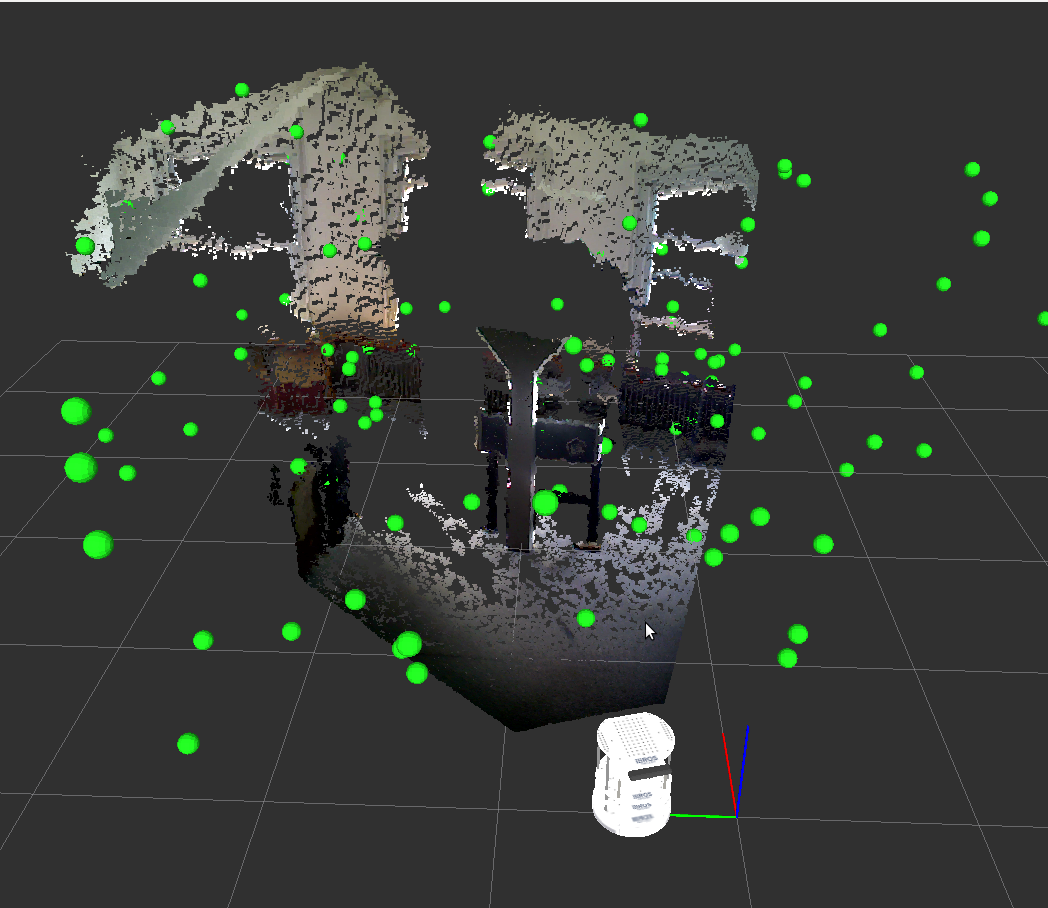
\includegraphics[width=.8\textwidth]{slam110landmarks2}
    \caption{SLAM session using the pipeline.}
  \label{slam}
\end{figure}


\subsubsection{Speed}

The speed factor was tested on a mid level as well as on a high level machine to see the differences in time needed to perform the operations. The results of a machine running on a pentium i5-3210M and on a pentium i7 are shown in table \ref{bench}:

\begin{center}

    \begin{tabular}{|C|C|C|C|C|C|}
    \hline
    \multicolumn{6}{|l|}{\centerline{Pentium i5-3210M}} \\
    \hline
     Leaf Size & Downs Time & Cloud size & Sampling & Matching,old & Matching,new \\
     \hline
     1m & 0.908768 & 9 & 0.0290296 & 0.00218081 & 0.00218081 \\
     \hline
     50cm & 0.914169 & 32 & 0.0112929 & 0.00154852 & 0.00243211 \\
     \hline
     30cm & 1.07862 & 79 & 0.0138666 & 0.00126673 & 0.00126673 \\
     \hline
     10cm & 1.1764 & 654 & 0.0712596 & 0.00154977 & 0.00154977 \\
     \hline 
     5cm & 1.75907 & 2391 & 0.215594 & 0.00181846 & 0.00181846 \\
     \hline
     1cm & 14.3283 & 25556 & 5.06356 & 0.00278712 & 0.854803  \\
     \hline
     \multicolumn{6}{|l|}{\centerline{Pentium i7-3610QM}} \\
     \hline
      Leaf Size & Downs Time & Cloud size & Sampling & Matching,old & Matching,new \\
      \hline
      1m &0.675993	&7&	-	&-&	-\\
      \hline
      50cm &0.779975&	30&	-&	-&	-\\
      \hline
      30cm &0.676315&	66&	-&	-&	-\\
      \hline
      10cm &0.746999&	488&	-&	-&	-\\
      \hline 
      5cm &0.878036&	1827&	0.132831&	0.00281951&	0.00281951\\
      \hline
      1cm &1.11554	&18487&	2.69855	&0.0021291	&0.0021291  \\
      \hline
	 \end{tabular}    
	 \label{bench}
\end{center}


The leaf size directly affects the time the cloud takes to be processed in the pipeline as well as the time the sampling takes aftewards. Experimental evaluation has showed that a leaf size between 1-5cm provides a good balance between speed and precision. The difference between Matching,old and Matching,new has to do with the fact that in the second case, a new landmark is added and therefore DB operations take place. When matching old is the same as matching new, then all the clusteres where matched to items in the database.

\subsubsection{Memory requirements}

The memory requirements of the method is a function that is directly affected to the $\alpha$ strength parameter of the sampler given that the decision boundary is constant. As the $\alpha$ parameter increases, the sampler will output more clusters on every iteration. The higher amount the of cluster will result a higher amount of landmarks and, consequently, in larger memory requirements in the method. Fig.\ref{memReq} shows memory requirements as a function of strength parameter alpha.


\begin{figure}[ht!]
  \centering
    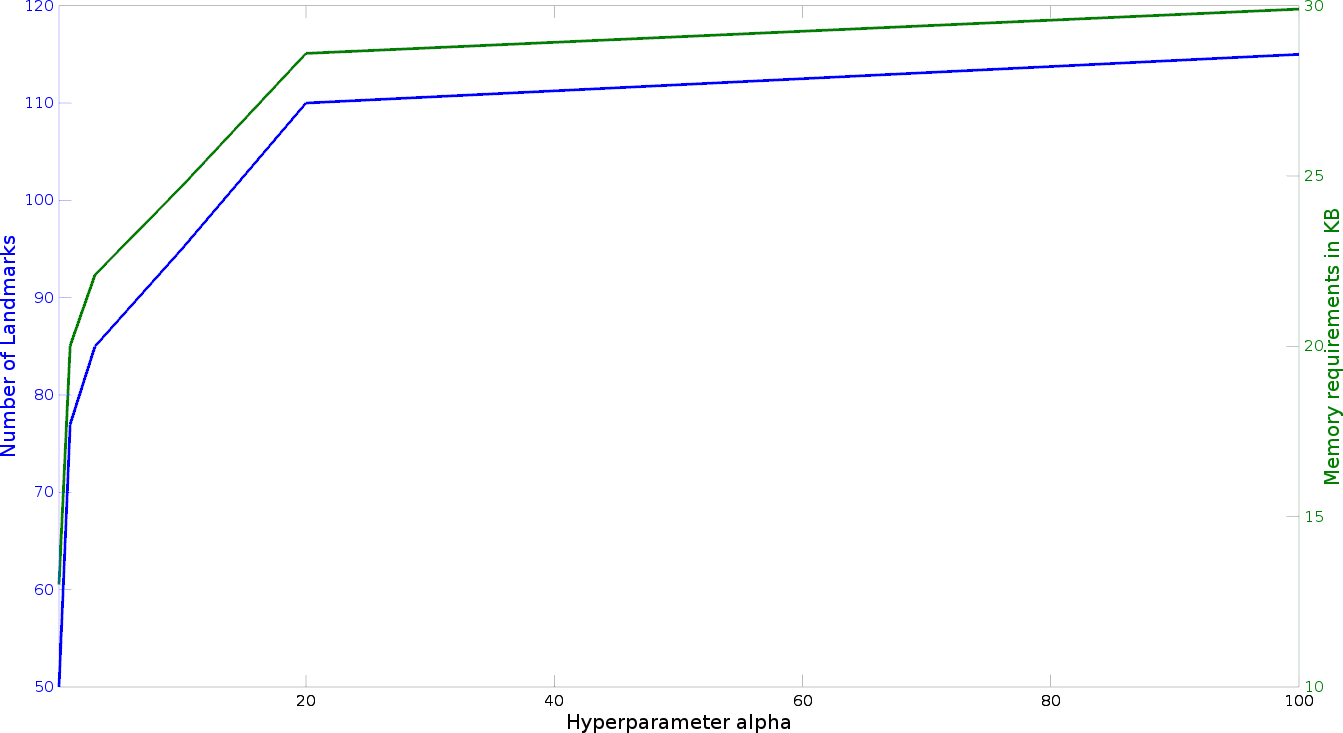
\includegraphics[width=.8\textwidth]{memoryRequirements2}
    \caption{Memory Requirements as a function of strength parameter $\alpha$.}
  \label{memReq}
\end{figure}

As it can be seen, the number of landmarks follows the logarithmic trend of the distribution in relation to $\alpha$. Increasing the alpha value more will not make the algorithm follow the logarithmic trend indefinitely. That is due to the fact that as the alpha increases, the constant decision layer has an upper bound to the number of landmarks it can have. This means that the algorithm will keep adding landmarks until the environment saturates and no new landmarks can be added. It must also be noted that as the alpha parameter is set to higher numbers, the sampler outputs more clusters making it more accurate of the environment descriptor it outputs, but also takes more time, making it non feasible to use this in real time mapping scenarios. Values of alpha between 0 and 10 provide a robust but also fast enough sampler that can be used in online mapping scenarios.



\section{Conclusion and future work}
\label{sec:discussion}

 In this paper a novel method for cloud representation using non-parametric Bayesian tools was introduced. Its strengths and weaknesses where presented and an application on how this method could be used to tackle the compression problem of long term SLAM were given. There is a number of directions in which such methods could be improved. Choosing more complex environment representations could increase the expresional stregth of the sampler making it easier to represent with better precision more complex objects. Furthermore, since the sampler clusters parts of environment, it would be interesting to see how a hierarchical approach would change the result of the clustering. Hierarchical dependent Dirichlet processes would be interesting extensions since such tools would both have the ability to capture structures instead of parts of the environment as well as be able to handle the dynamic component that long term slam problems introduce. Furthermore, having a more complex decision layer would also increase the robustness of the method making it able to handle more complex environment structures. Finally, all those additions could help lift the dynamic environment restrictions that were defined in Walcotts PhD thesis and make the pipeline handle in a fully Bayesian way the long term mapping implications of SLAMa
 
%------------------------------------------------

\begin{thebibliography}{9}

\bibitem{probRobs}
\newblock Thrun, S. (2002). Probabilistic robotics. Communications of the ACM, 45(3), 52-57.


\bibitem{ekf}
\newblock Bailey, T., Nieto, J., Guivant, J., Stevens, M., \& Nebot, E. (2006, October). Consistency of the EKF-SLAM algorithm. In Intelligent Robots and Systems, 2006 IEEE/RSJ International Conference on (pp. 3562-3568). IEEE.

\bibitem{graph}
\newblock Thrun, S., \& Montemerlo, M. (2006). The graph SLAM algorithm with applications to large-scale mapping of urban structures. The International Journal of Robotics Research, 25(5-6), 403-429.

\bibitem{Figueredo:2009dg}
Figueredo, A.J. and Wolf, P. S.A. (2009).
\newblock Assortative pairing and life history strategy - a cross-cultural
  study.
\newblock {\em Human Nature}, 20:317--330.

\bibitem{liflonglearning}
\newblock Thrun, S., \& Mitchell, T. M. (1995). Lifelong robot learning. The Biology and Technology of Intelligent Autonomous Agents, 165-196.

\bibitem{lifelongmaps}
\newblock Konolige, K., \& Bowman, J. (2009, October). Towards lifelong visual maps. In Intelligent Robots and Systems, 2009. IROS 2009. IEEE/RSJ International Conference on (pp. 1156-1163). IEEE.

\bibitem{aishalong}
\newblock Walcott, A. (2011). Long-term robot mapping in dynamic environments (Doctoral dissertation, Massachusetts Institute of Technology).

\bibitem{bayesianNon}
\newblock Hjort, N. L., Holmes, C., Müller, P., \& Walker, S. G. (Eds.). (2010). Bayesian nonparametrics (Vol. 28). Cambridge University Press.

\bibitem{dependent}
\newblock {MacEachern, S. N. (2000) Dependent dirichlet processes. Unpublished manuscript, Department of Statistics, The Ohio State University.}

\bibitem{brml}
\newblock{Barber, D. (2012) Bayesian reasoning and machine learning.}

\bibitem{dependentDiri}
\newblock{Neiswanger, W., Wood, F., \& Xing, E.The dependent dirichlet process mixture of objects for detection-free tracking and object modeling. In Proceedings of the Seventeenth International Conference on Artificial Intelligence and Statistics (pp. 660-668) (2014, August) }

\bibitem{pcl}
\newblock{Rusu, R. B., \& Cousins, S. (2011, May). 3d is here: Point cloud library (pcl). In Robotics and Automation (ICRA), 2011 IEEE International Conference on (pp. 1-4). IEEE.}

\bibitem{rtabmap}
\newblock Labbé, M., \& Michaud, F. (2011, September). Memory management for real-time appearance-based loop closure detection. In Intelligent Robots and Systems (IROS), 2011 IEEE/RSJ International Conference on (pp. 1271-1276). IEEE.


\bibitem{slam++}
\newblock Salas-Moreno, R. F., Newcombe, R. A., Strasdat, H., Kelly, P. H., \& Davison, A. J. (2013, June). Slam++: Simultaneous localisation and mapping at the level of objects. In Computer Vision and Pattern Recognition (CVPR), 2013 IEEE Conference on (pp. 1352-1359). IEEE.

\bibitem{objslam}
\newblock Selvatici, A. H., \& Costa, A. H. (2008). Object-based visual slam: How object identity informs geometry.

\bibitem{castleetal}
\newblock Castle, R. O., Gawley, D. J., Klein, G., \& Murray, D. W. (2007, April). Towards simultaneous recognition, localization and mapping for hand-held and wearable cameras. In Robotics and Automation, 2007 IEEE International Conference on (pp. 4102-4107). IEEE.


\bibitem{objectpointslam}
\newblock Choudhary, S., Trevor, A. J., Christensen, H. I., \& Dellaert, F. (2014, September). SLAM with object discovery, modeling and mapping. In Intelligent Robots and Systems (IROS 2014), 2014 IEEE/RSJ International Conference on (pp. 1018-1025). IEEE.

\bibitem{objectpoint}
\newblock Jensfelt, P., Ekvall, S., Kragic, D., \& Aarno, D. (2006, September). Augmenting slam with object detection in a service robot framework. In Robot and Human Interactive Communication, 2006. ROMAN 2006. The 15th IEEE International Symposium on (pp. 741-746). IEEE.

\bibitem{monoslam}
\newblock Davison, A. J., Reid, I. D., Molton, N. D., \& Stasse, O. (2007). MonoSLAM: Real-time single camera SLAM. Pattern Analysis and Machine Intelligence, IEEE Transactions on, 29(6), 1052-1067.

\bibitem{objectDisc}
\newblock Koo, S., Lee, D., \& Kwon, D. S. (2014, September). Unsupervised object individuation from RGB-D image sequences. In Intelligent Robots and Systems (IROS 2014), 2014 IEEE/RSJ International Conference on (pp. 4450-4457). IEEE.


\bibitem{distMes}
\newblock{Cichocki, A., \& Amari, S. I.Families of alpha-beta-and gamma-divergences: Flexible and robust measures of similarities. Entropy, 12(6), 1532-1568.}

\bibitem{fpfh}
\newblock{Fast point feature histogram.Rusu, R. B., Blodow, N., \& Beetz, M. (2009, May). Fast point feature histograms (FPFH) for 3D registration. In Robotics and Automation, 2009. ICRA'09. IEEE International Conference on (pp. 3212-3217). IEEE.}

\bibitem{segOverview}
\newblock {Rabbani, T., van den Heuvel, F., \& Vosselmann, G. (2006). Segmentation of point clouds using smoothness constraint. International Archives of Photogrammetry, Remote Sensing and Spatial Information Sciences, 36(5), 248-253.}

\bibitem{gpu}
\newblock{Caron, F., Davy, M., \& Doucet, A. (2012) Generalized Polya urn for time-varying Dirichlet process mixtures. arXiv preprint arXiv:1206.5254.}


\bibitem{kinect}
\newblock{Zhang, Z. (2012) Microsoft kinect sensor and its effect. MultiMedia, IEEE, 19(2), 4-10.}

\bibitem{nonParam}
\newblock{Wainwright, M. J., \& Jordan, M. I. (2008). Graphical models, exponential families, and variational inference. Foundations and Trends in Machine Learning, 1(1-2), 1-305.}
``
\bibitem{omnimaper}
\newblock{A.Trevor,  J.Rogers, and  H.Christensen.  Omnimapper:  A  modular multimodal  mapping  framework.   In IEEE  International  Conference on Robotics and Automation (ICRA), 2014}

\bibitem{imft}
\newblock Koo, S., Lee, D., \& Kwon, D. S. (2013, November). Multiple object tracking using an rgb-d camera by hierarchical spatiotemporal data association. In Intelligent Robots and Systems (IROS), 2013 IEEE/RSJ International Conference on (pp. 1113-1118). IEEE.

\bibitem{pointSeg}
\newblock Trevor, A. J., Gedikli, S., Rusu, R. B., \& Christensen, H. I. (2013). Efficient organized point cloud segmentation with connected components. Semantic Perception Mapping and Exploration (SPME).

\bibitem{planarSeg}
\newblock Unnikrishnan, R., \& Hebert, M. (2003, October). Robust extraction of multiple structures from non-uniformly sampled data. In Intelligent Robots and Systems, 2003.(IROS 2003). Proceedings. 2003 IEEE/RSJ International Conference on (Vol. 2, pp. 1322-1329). IEEE. 

\bibitem{planarSeg2}
\newblock Rabbani, T., van den Heuvel, F., \& Vosselmann, G. (2006). Segmentation of point clouds using smoothness constraint. International Archives of Photogrammetry, Remote Sensing and Spatial Information Sciences, 36(5), 248-253.

\bibitem{smartSeg}
\newblock Triebel, R., Shin, J., \& Siegwart, R. (2010, June). Segmentation and unsupervised part-based discovery of repetitive objects. In Robotics: Science and Systems (Vol. 2).

\bibitem{smcddp}
\newblock Neiswanger, W., Wood, F., \& Xing, E. (2014, August). The dependent dirichlet process mixture of objects for detection-free tracking and object modeling. In Proceedings of the Seventeenth International Conference on Artificial Intelligence and Statistics (pp. 660-668).

\bibitem{corresp:first}
\newblock Cree, M. J., Jefferies, M. E., \& Baker, J. T. Using 3D Visual Landmarks to Solve the Correspondence Problem in Simultaneous Localisation and Mapping.

\bibitem{corres:sec}
\newblock Lowe, D. G. (2004). Distinctive image features from scale-invariant keypoints. International journal of computer vision, 60(2), 91-110.

\bibitem{corres:three}
\newblock Lamon, P., Tapus, A., Glauser, E., Tomatis, N., \& Siegwart, R. (2003, October). Environmental modeling with fingerprint sequences for topological global localization. In Intelligent Robots and Systems, 2003.(IROS 2003). Proceedings. 2003 IEEE/RSJ International Conference on (Vol. 4, pp. 3781-3786). IEEE.


\bibitem{corres:four}
\newblock Sehgal, A., Cernea, D., \& Makaveeva, M. (2010). Real-time scale invariant 3D range point cloud registration. In Image Analysis and Recognition (pp. 220-229). Springer Berlin Heidelberg.

\bibitem{bayes:neal}
\newblock Neal, R. M. (2000). Markov chain sampling methods for Dirichlet process mixture models. Journal of computational and graphical statistics, 9(2), 249-265.

\bibitem{bayes:jordan}
\newblock Blei, D. M., \& Jordan, M. I. (2006). Variational inference for Dirichlet process mixtures. Bayesian analysis, 1(1), 121-143.

\bibitem{slam}
\newblock{Montemerlo, M., Thrun, S., Koller, D., \& Wegbreit, B. (2002). FastSLAM: A factored solution to the simultaneous localization and mapping problem. AAAI/IAAI, 593-598.}

\bibitem{bayes:hier}
\newblock Teh, Y. W., Jordan, M. I., Beal, M. J., \& Blei, D. M. (2006). Hierarchical dirichlet processes. Journal of the american statistical association, 101(476).

\bibitem{bayes:smc}
\newblock Doucet, A., De Freitas, N., \& Gordon, N. (2001). An introduction to sequential Monte Carlo methods (pp. 3-14). Springer New York.

\bibitem{LDA}
\newblock{Blei, D. M., Ng, A. Y., \& Jordan, M. I. (2003). Latent dirichlet allocation. the Journal of machine Learning research, 3, 993-1022.}

\bibitem{theory:ddp}
\newblock MacEachern, S. N. (2000). -
\bibitem{speakerDiar}
\newblock{Fox, E. B., Sudderth, E. B., Jordan, M. I., \& Willsky, A. S. (2011). A sticky HDP-HMM with application to speaker diarization. The Annals of Applied Statistics, 5(2A), 1020-1056.}


\bibitem{antoniak}
\newblock{Charles E Antoniak,Mixtures of dirichlet processes with applications to bayesian nonparametric problems, The annals of statistics (1974), 1152–1174}

\bibitem{caron}
\newblock{F. Caron, M. Davy, and A. Doucet, Generalized Polya urn for time-varying Dirichlet process mixtures, 23rd Conference on
Uncertainty in Artificial Intelligence (UAI’2007), Vancouver,
Canada, July 2007, 2007}

\bibitem{compendium}
\newblock{Fink, D. (1997). A compendium of conjugate priors.}

\bibitem{smc:theory}
\newblock{Ülker, Y., Günsel, B., \& Cemgil, A. T. (2010). Sequential Monte Carlo samplers for Dirichlet process mixtures. In International Conference on Artificial Intelligence and Statistics (pp. 876-883).}

\bibitem{doucet}
\newblock{Del Moral, P., Doucet, A., \& Jasra, A. (2006). Sequential monte carlo samplers. Journal of the Royal Statistical Society: Series B (Statistical Methodology), 68(3), 411-436.}

\bibitem{RANSAC}
\newblock{Meer, P., Mintz, D., Rosenfeld, A., \& Kim, D. Y. (1991). Robust regression methods for computer vision: A review. International journal of computer vision, 6(1), 59-70.}

\bibitem{conjugate}
\newblock Raiffa, H. (1974). Applied statistical decision theory.

\bibitem{sqlite}
\newblock{https://www.sqlite.org/datatype3.html}

\bibitem{polya}
\newblock{Johnson, N. L., \& Kotz, S. (1977). Urn models and their application: an approach to modern discrete probability theory (Vol. 77). New York: Wiley.}

\end{thebibliography}

%----------------------------------------------------------------------------------------



\end{document}
